\graphicspath{{chapters/4.Chapter_2/figures/}}

\begin{savequote}[75mm]
"even after the observation of the frequent or constant conjunction of objects, we have no reason to draw any inference concerning any object beyond those of which we have had experience;"
\qauthor{- David Hume: \textit{A Treastie of Human Nature, 1738}}
\end{savequote}

\chapter{Transcriptomic analysis of the \textit{Paramecium bursaria} and \textit{Micractinium reisseri} endosymbiosis}

%%%% INCORPORATE UPDATED CLEANED ML SHIT (REMOVING SHITTY TRAINING)
%%%% REDO BINNING ON HMMSCAN AND PFAM ANALYSIS WITH RECALLED ORFS - REMOVING 

\section{Introduction}

The \textit{Paramecium bursaria}-\textit{Micractinium reisseri} (PbMr) endosymbiosis 
conveys phototrophy \citep{Karakashian1963}, numerous photobiological traits (e.g. \citep{Berk1991,Saji1974,Nakajima1989,Niess1982a,Iwatsuki1988,Summerer2009}, 
partially reviewed in \citep{Sommaruga2009}) and its establishment and maintenance 
is dependent on photosynthetic activity and enigmatic light-induced factors \citep{Karakashian1963,Hosoya1995a,Kodama2007,Kodama2014c}.
Therefore, a relatively unbiased global metatranscriptomic profile of host and endosymbiont in both lit and dark conditions 
would potentially identify key transcripts which play a role in the establishment, maintenance, and characteristics 
of this endosymbiosis. 


``Dual-RNAseq'' is a form transcriptomics which characterises transcripts in a small number of defined organisms simultaneously \citep{Westermann2012}.
It has proven an effective method in several studies investigating host-chloroplast interactions \citep{Nowack2011,Jiggins2013,Xiang2015},
and host-pathogen systems \citep{Tierney2012,Kawahara2012,Jones2014,Hayden2014}.
It differentiates itself from both standard metatranscriptomics, such as those common in microbial ecology \citep{Poretsky2005,AliagaGoltsman2014},
by being conducted on samples of known, or mostly known composition, and from classical transcriptomics
by not depending on axenic samples. 


\textit{Paramecium bursaria} and its green algal endosymbionts form a system well-posed
for ``dual-RNAseq'' analysis.  Firstly, there is a plethora 
of literature on the physiology and behaviour of host and endosymbiont, both together and individually
(e.g. \citep{Iwatsuki1988}, see \citep{Kato2009a} and the Introductory Chapter for more details), presenting 
a key resource by which results can be contextualised.
Additionally, transcriptomic analysis has proven feasible in reasonably close relatives of both host \citep{Arnaiz2010,Kolisko2014} and endosymbiont \citep{Guarnieri2011,Rowe2014,Bashan2015}.  
Even more promisingly, there has been an analysis of the host-endosymbiont
system (although in a different strain: Yad1g1N) \citep{Kodama2014}. 
Unfortunately, this study focused only on the expression pattern of the host
alone with and without its endosymbiont and discarded endosymbiont derived data
during analysis.


This said, the PbMr system does also present some severe difficulties in terms of its transcriptomic tractability.
Specifically, the system is highly genomically and transcriptomically complex with \textit{P. bursaria}'s ciliate nuclear
dimorphism and high order polyploidy \citep{Raikov1995}, 
the presence of sexual reproduction in both host \citep{Jennings1939} and endosymbiont species \citep{Blanc2010},
and a large range of GC biases \citep{Kodama2014}. Therefore, care must be taken to optimise sequencing,
and assembly methods to mitigate these complications.


These difficulties are compounded by the lack of available reference genomes for either \textit{Paramecium bursaria} or \textit{Micractinium reisseri} and thus necessitating \textit{de novo} transcriptome assembly.
However, the utility of sequenced genomes from divergent ciliate species 
(i.e. \textit{Tetrahymena thermophila} \citep{Eisen2006}, \textit{Paramecium tetaurelia} \citep{Aury2006} and \textit{Paramecium caudatum}
\citep{McGrath2014}) and endosymbiotic green algae \textit{Chlorella variabilis} NC64A \citep{Blanc2010} and \textit{Coccomyxa subellipsoidea} C-169 \citep{Blanc2012}
(see \cref{fig:paramecium_genomes} in the Introductory Chapter and \cref{fig:its2_phylo} in Chapter 3 for respective phylogenetic context of these genomes) as references for assembly was investigated.
It should also be noted that the existing \textit{Paramecium bursaria} \citep{Kodama2014}, 
\textit{Paramecium duboscqui} \citep{Kolisko2014} and
\textit{Chlorella vulgaris} \citep{Guarnieri2011} transcriptomes mentioned above were
successfully recapitulated \textit{de novo} (without a reference genome).


The mixotrophic nature of the host \textit{Paramecium} \citep{Dolan1992} means there 
are partially digested bacterial prey species, as well as numerous 
associated bacteria \citep{Gortz2009,Fokin2009,Schrallhammer2009} and viruses \citep{VanEtten1983} which
all present potentially obfuscating sources of contamination in the analysis of host-endosymbiont
interaction.  
Therefore, it is key to effective analysis of this system to develop methods
to minimise the effects of contamination at all stages of analysis.  To address this,
we investigated methods to reduce contamination during library preparation such as washing steps, cell picking
and single cell sequencing techniques; methods to screen and/or filter sequenced libraries
for contaminants before inclusion in assembly and methods to effectively sort
assembled transcripts into bins relating to their likely originating organisms
(i.e. ``host'', ``food'' or ``endosymbiont'' derived).



To this end, bulk RNAseq libraries from cultured PbMr was sequenced using 76bp paired-end reads and the Illumina Gene Analyzer II platform 
taking care to minimise contamination by filtering and washing cultures and carefully
assessing culture health to maximise the number of healthy PbMr sequenced. 
Unfortunately, due to limitations in the maintainable culture density of the 
\textit{Paramecium bursaria} CCAP 1660/12 and thus the quantity of extractable
mRNA it was necessary to pool all day and night replicates into a single pair of day and night libraries. 

While this provided sufficient material for sequencing it precluded accurate inference of differential expression between day or night
by masking the biological replicates \citep{Auer2010}.
We, therefore, also sequenced a set of 3 (followed later by an additional 5) dark and 3 light
biological replicates using single-cell RNAseq (sc-RNAseq) methods.
This also allowed a finer-grain control over cell selection and potentially
a method to reduce culture based contamination.


While reasonably nascent, sc-RNAseq has shown a lot of promise in well characterised systems such as human cell cultures \citep{Bengtsson2005,Shalek2013}
and \textit{Saccharomyces cerevisiae} \citep{Lipson2009} and there are high expectations
of their utility for ``dual-RNASeq'' \citep{Westermann2012}.  sc-RNAseq addresses 
the key difficulties of analysing unculturable or poorly culturable organisms \citep{Murray2012} and investigating
cell-cell heterogeneity in expression patterns \citep{Raj2008,Shalek2013}).  
Uninvestigated, this heterogeneity (either from biological and/or genomic variance or just the stochasticity of gene expression),
can lead to a Yule-Simpson effect \citep{Yule1903a,Simpson1951}, where the false amalgamation of distinct expression patterns
in previously cryptic but distinct cellular subpopulations could generate a spurious expression pattern contrary to either subpopulation.


There are a range of possible sc-RNAseq methods (whose advantages and disadvantages are covered in the Methods Chapter).
We used Qiagen's Repli-G Whole Transcriptome Amplification (WTA) MDA-based kit as MDA 
is well established and characterised in single cell genomics (e.g. \citep{Spits2006}), 
has a simple methodology not requiring additional equipment, and is potentially more successful at
recovering transcripts from a wide range of abundance levels than other methods i.e. recovers many lowly expressed transcripts\footnote{\hfill\url{https://www.qiagen.com/gb/shop/sample-technologies/rna-sample-technologies/total-rna/repli-g-wta-single-cell-kit/} as of 2015/08/25}.
Unfortunately, despite the publication of empirical comparisons of single cell transcriptomic methods \citep{Wu2014a}, 
Qiagen's Repli-G WTA MDA-based kit has yet to be directly assessed relative to other approaches and thus its performance has not
been independently verified. 
Briefly, this method involves the ligation of reverse transcribed cDNAs using oligo-dT primers (after lysis and 
removal of gDNA) before MDA by a \(\phi29\) DNA polymerase with a 5'-3' exonuclease proofreading activity 
(reducing error-rate of amplification to \(9.5\cdot10^{-6}\) errors per nucleotide \citep{Paez2004} compared with
\(10^{-4}\) to \(10^{-5}\) for Taq \citep{Tindall1988,Eckert1990}) \citep{Korfhage2015}.



Unfortunately, despite its utility sc-RNAseq generates a new set of difficulties.
First and foremost, there has only been a single published use of sc-RNAseq, to my knowledge, in non-model unicellular eukaryotes.   
This study by \citep{Kolisko2014}, briefly addressed the issues of bias, contamination and gene discovery effectiveness in a set of model and non-model eukaryotes and
constitutes an important proof-of-concept.  
However, it also used a different sc-RNAseq approach (SMART), focused on single organisms, 
and didn't address, in-depth, the optimal way to process, assemble and utilise single cell datasets from protists.
While some work has been done investigating the optimal pre-processing of bulk RNAseq datasets (e.g. \citep{Macmanes2013,Macmanes2015}) 
the effect of different trims and error correction on sc-RNAseq has yet to be characterised.  
There are also some early indications of problems of cryptic bacterial contamination
from samples and/or reagents in sc-RNAseq is particularly problematic \citep{Kolisko2014}. 
This further increases the importance of library screening and post-assembly transcript binning.

\section{Aims}
Therefore, this chapter will investigate the optimal use of 2nd generation bulk and sc-RNAseq libraries
in a characterising a complex reference-free system.  Specifically, it will look at the screening of RNAseq libraries for contamination
before assembly, the optimal preprocessing (partitioning, trimming, digital normalisation and error correction), assembler and assembly
parameters (including the utility of divergent reference genomes from related species) in recapitulation of host and endosymbiont transcripts.
Finally, I will address the problem of the attribution of recovered transcripts into their appropriate likely originating organism.  
\section{Methods} 

\subsection{Sample preparation and sequencing}

\subsubsection{Bulk transcriptome RNA preparation}
For bulk transcriptomic analyses CCAP 1660/12 cells were harvested in a way to minimise 
contamination from bacterial prey species in the culture. \(\sim 10^{6}\) 
cell aliquots were strained through \(40\mu m\) sieves, filtered on 
\(10 \mu m\) nylon filters, 
before finally being filtered on \(8 \mu m\) TETP polycarbonate filters using a 
low-pressure filtration pump.  Collected samples were either immediately 
quick-frozen in liquid nitrogen for storage (\(-20\)\celsius for short-term storage 
and \(-80\)\celsius for longer storage) or harvested by centrifugation.  
In order to investigate the two main metabolic states of the symbiosis 
(i.e. under light conditions during active photosynthesis and in the dark 
when no photosynthesis is taking place) samples were extracted 5 hours into 
the light and dark phase of the 12:12 hour day-night cycle.

To ensure extracted RNA was representative of healthy and interacting host 
and endosymbionts care was taken to the number of dead/dying cells 
from which RNA was extracted.  In order to do this, a subsample was taken 
from each culture during the process of harvesting and scored for dead/dying cells.  
Cell assays were formed by taking 1-2ml of each harvest cell pellet and 
fixed using 40\(\mu l\) Lugol's solution (0.5g \(I_{2}\) and 1g KCl in 8.5ml 
of MilliQ water). Dead/dying cells were identified as broken or puckered cells 
and counted using light microscopy.  Samples containing >10\% dead/dying cells 
were discarded and no RNA extracted from them.

In order to lyse collected samples, cells were washed from the filter or the 
pellet was resuspended in 1ml TriReagent (Sigma) heated to \(60\)\celsius. 
Cells were vortexed with sterile \(300\mu m\) glass-beads for 15s, incubated at 
room temperature for 10 minute, vortexed for 15s, quick-frozen in liquid 
nitrogen and stored at \(-20\celsius\)
before further processing.  
Samples were defrosted, vortexed for 15s, placed in a heat-block set 
to \(60\celsius\) 
for 10 minutes while continuing to be vortexed, removed from 
heating and vortexed again for 15s.  
RNA was extracted by adding 0.2ml of Chloroform to the glass-bead-trizol-sample 
solution, shaking for 15s, incubating for 5 minutes at room temperature and 
centrifuging at 12,000g for 15 minutes at 4\celsius.  
The upper-phase was then transferred to an RNAse-free 1.5ml tube and an 
equal volume (\(\sim0.5ml\)) of isopropanol was added before shaking for 15s.  
The isolated RNA was then incubated at \(-20\)\celsius for 10 minutes 
(up to several hours) before being collected as a pellet using a centrifuge at 
10,000g for 10 minutes at \(4\celsius\)
(supernatant was discarded). 
The RNA pellet was then washed with 1ml of 75\% ethanol and centrifuged 
twice at 10,000g for 10 minutes at 4\celsius with the supernatant being 
discarded after each centrifugation.  
The pellet was then dried before being resuspended in \(100\mu l\) of RNAse-free water.  
The RNA was cleaned further using the Qiagen RNeasy clean-up kit 
before being assessed for quality using ND-1000 (NanoDrop) and BioAnalyzer (Agilent).

\subsubsection{Single cell RNA preparation}
For single cell transcriptomics, a ``cell-picking'' approach was used in which
\textit{P. bursaria} cells (from the CCAP1660/12 culture) were inspected on an inverted light microscope 
before being picked using an orally aspirated drawn-glass Pasteur pipette \citep{Garcia-Cuetos2012}.
In order to minimise contamination from food bacteria present in the media these picked cells
were washed 3 times by serial transfer to \(10\mu l\) droplets of sterile NCL media.
The washed cell was then transferred to a \(10\mu l\) droplet of sterile water.
Cells were picked 5 hours into both the lit and dark phase of the 12:12 hour day-night cycle 
identically to the bulk analyses.
As cells were picked individually, health status could be exhaustively assessed
during picking and therefore the subsampling and scoring method used to
check the status of cells in bulk preparations was unnecessary.

cDNA was generated and amplified using the MDA-based Qiagen REPLI-g WTA Single Cell Kit \citep{Korfhage2015}
with additional cell disruption steps. 
Specifically, cells were transferred from their respective \(10\mu l\) droplets of sterile water to
a PCR tube containing \(6\mu l\) water and \(4\mu l \) lysis buffer. 
Due to the robust chitin cell walls of \textit{M. reisseri} \citep{Kapaun1995} it was important to
ensure thorough cell lysis. Therefore, samples underwent mechanical disruption by bead beating (Sigma, \(425-600\mu m\), acid-washed)
followed by freeze-thaw via submersion in liquid nitrogen for 5 seconds.
In order to compare disruption methods, extractions and amplifications
were also conducted using just lysis buffer, bead beating and vortexing (i.e. without freeze-thaw), 
and just the lysis buffer.  Samples were then quantified using a ND-1000 (NanoDrop)
and as extraction methods produced near identical DNA concentrations 
the maximal disruptive method of freeze-thaw, beat beating, vortexing and lysis buffer
described above was used for further purification and library preparation.
The samples were then vortexed for 1 minute before a gDNA removal step.

mRNA was selectively amplified and reverse transcribed to cDNA using poly-A selection (i.e. oligo-dT) primers
to prevent amplifying ribosomal sequences. Prior to MDA by a \(\phi29\) DNA polymerase
cDNA were ligated into long fragments due to lower MDA efficiency for short fragments \citep{Korfhage2015}.
This reduces size-dependent amplification bias but could potentially lead to the creation
of chimeric transcripts in which paired-reads cross boundaries of adjacently ligated
cDNA transcripts.  Analysis of this is discussed below.

The amplified cDNA was then purified using a QIAamp DNA mini kit and eluted in \(100\mu l\) elution buffer.
This kit operates by binding the DNA to a QIAmp membrane in a spin column followed by successive washing steps
to remove impurities such as remaining proteins and cations. To create 3 dark cDNA 
samples (Dark1-2, Dark1-3, Dark1-5) and 3 light samples (Light1-9, Light1-10, Light1-11).


Due to low quantities of eukaryote identifiable reads in the initial 3 sequenced single cell
dark libraries a set of additional single cell extractions were conducted. 
These followed the same protocol as above but also featured an additional
final PCR-based screening of synthesised cDNA using primers specific for \textit{Paramecium}
Bug22 sequence. Bug22 is a highly conserved ciliary protein found in a large number of organisms
including the ciliates \citep{Smith2005,Laligne2010}, green algae \citep{Keller2005,Laligne2010,Meng2014}, higher plants \citep{Hodges2011}, and animals \citep{MendesMaia2014} we used as a marker for \textit{Paramecium} derived cDNA.
Primers used were Bug22BFWD "GCATTCTAGACCAATCTGGCTTTCTGTCAA" and Bug22BREV "GCATTTCGAATTTGAGGCTCTAAATCTTCTTCTCA",
under standard PCR conditions.  5 (Dark2-2, Dark2-3, Dark2-6, Dark2-7, Dark2-8) samples with 
bands of appropriate size were then taken forward for library preparation and sequencing.


\subsubsection{Library preparation}

For both bulk and single cell preparations each cDNA sample was fragmented in \(130\mu l\) 1xTE buffer on the Covaris E220 
with a target size of \(225bp\) (duty factor of \(10\%\), 200 cycles per burst, peak incident power
of 175, \(200s\) at \(7^{o}C\)). Fragment sizes were checked on a BioAnalyzer (Agilent) 7500 DNA chip.
cDNA was then concentrated using a GeneRead kit column with a elution in \(35\mu l\). Fragmentation
step was then repeated 3 times (\(110s\)) until majority of cDNA in each library was between \(200-250bp\)

cDNA ends were then end-repaired, adenylated and adapters ligated using the NEXTFlex (Biooscientfic) sequencing kit 
according to the manufacturer's instructions and using NEBNext (New England Biolabs) indices.  Also following
the NEXTFlex kit instructions, MgNa bead purification was done before and after PCR amplification using
NEBNext reagents.  Finally, prepared libraries were size selected using a Blue Pippin machine at a size selection
of \(350bp\) (range \(315-385bp\)).

A final bioanalyzer step was conducted with individual library concentrations ranging from \(0.66-4.09nM\).


\subsubsection{Sequencing}

The bulk day and night library were paired-end (PE) \(76bp\) sequenced using an Illumina Genome
Analyzer II by the Exeter University Sequencing Service.  The two libraries were sequenced
on separate flowcells (Bulk-Light, Bulk-Dark).

Single cell libraries were paired-end \(150bp\) using an Illumina HiSeq 2500 by Exeter
Sequencing Service. 3 dark (Dark1-2, Dark1-3, Dark1-5) and 3 light (Light1-9, Light1-10, Light1-11)
samples were multiplexed sequenced on a single flowcell lane.  The 5 additional 
dark samples (Dark2-2, Dark2-3, Dark2-6, Dark2-7, Dark2-8) were multiplexed and sequenced on a single
flowcell lane in a separate sequencing run.

\subsection{Library contamination screening}

\subsubsection{Taxonomic analysis}
Sequenced libraries were initially screened using the standard
metrics implemented in the FastQC to check for standard sequencing issues
such as flowcell defects, library degradation, and adapter read-through \citep{fastqc2015}.

To further investigate potential contamination, a taxonomic
profile and GC\% probability density was determined for each library.

The former was conducted using a custom tool dubbed ``DueyDrop'' which functions as follows.
Briefly, for each library 5 batches of 10,000 PE reads were sampled 
using the reservoir sampler \citep{Vitter1985} implemented in Heng Li's seqtk library \citep{SeqtkGitHub}.
Despite 5 batches of 10,000 reads theoretically being equivalent to 50,000 random samples by splitting
sampling and using a different random seed any problems from poor randomisation implementation 
was minimised and consistency of taxonomic profiles could be easily assessed.
These randomly sampled reads were subsequently aligned to NCBI's Protein NR RefSeq database \citep{Pruitt2007}
using the efficient short-read optimised BLASTX implementation of DIAMOND \citep{Buchfink2015} (at a expectation
    of \(e^{-5}\) and top hits for each read retained.  Gene identifiers (GI) were extracted from these tops hits and queried against a
local copy of the NCBI taxonomy database \citep{Federhen2012} to recover a hit taxonomic lineage for each
read that aligned to a sequence within NR database. These lineages were then interactively tallied 
at several different taxonomic levels (e.g. domain level - eukaryote vs bacteria, or lower level - viridiplantae vs ciliate) and variances
calculated.  Results were then tabulated and libraries compared to assess whether any libraries appeared
aberrant.  This whole analysis was repeated for both untrimmed reads and reads quality trimmed
to a high quality threshold of an average Q30 over a sliding window of size 4 using
Trimmomatic \citep{Bolger2014a} to assess the impact trimming has on this profiling.
Taxonomic profiles were additionally visualised in Krona \citep{Ondov2011} using
the tabular BLAST hit import functionality.

Scripts used to conduct this analysis are available in the following github repository:\\
\url{https://github.com/fmaguire/dueydrop}

To determine how representative profiles created using small subsamples 
consisting of <1\% of reads are to profiles of entire libraries a similar analysis
was done using full libraries. All libraries were pre-trimmed at the harsh
threshold of the Q30 sliding window discussed above. 
The forward read from each trimmed library was used 
used in a similar DIAMOND based BLASTX search however all hits were retained.
Multiple hits for a given read were collapsed 
into a single lowest common ancestor (LCA) using the LCA algorithm \citep{Gabow1985} implemented in MEGAN (via the ``mtools''
package) \citep{Huson2007,el2013improved}.  LCA were then summarised and tabulated using
a script in the CGAT collections (``lca2table.py'') \citep{Sims2014} and visualised 
using Krona \citep{Ondov2011}.

On the basis of the resultant taxonomic profiles libraries were excluded or included
from downstream preprocessing and assembly. The libraries selected for inclusion during these analyses 
are referred to as the ``taxonomically filtered'' single cell libraries.

\subsubsection{GC density estimates}

Each library's GC\% probability density was estimated from per-read GC proportions
(calculated using awk \citep{Aho1987}) via Kernel Density Estimation (KDE) \citep{Rosenblatt1956,Parzen1962} 
(implemented in the seaborn package \citep{michael_waskom_2015_19108}).
This involved a standard gaussian kernel and a bandwith determined by ``Scott's normal reference rule'' \citep{Scott1979}.  
Again this analysis was repeated with both untrimmed and Q30 trimmed reads. 

\subsection{Optimising read pre-processing}

\subsubsection{Trimming}

To investigate the optimal trimming parameters for single cell libraries, 
random subsamples were trimmed using a range minimum quality thresholds and then the effects investigated
by mapping against 3 draft \textit{de novo} transcriptomes.

Specifically, 5000 PE reads were randomly sampled without replacement from each of the raw FASTQ libraries 
using the streaming reservoir sampling \citep{Vitter1985} algorithm implemented in Heng Li's 
seqtk C library (\citep{SeqtkGitHub}).
To guarantee that pairing was maintained the same random seed was used for the left and right read
of each library and incremented between libraries.

Trimmomatic \citep{Bolger2014a} was run on these samples with adapter clipping (ILLUMINACLIP)
using sequencing service provided fasta file of adapters, a maximum mismatch count of 2,
a palindromic clip threshold of Q35 and a simple clip threshold of Q15, a sliding window
quality trim of size 4 and average window quality thresholds of Q0, Q2, Q5, Q10, Q15, Q20, Q25, Q30, Q35, and Q40.
Finally, a minimum length trimmed read length criteria of 40bp was used.  


The trimmed samples were then mapped to 3 different \textit{de novo} draft transcriptome assemblies using bowtie2
\citep{Langmead2012} with maximum and minimum insert sizes of 37bp and 1161bp (derived from library preparation
fragment size distribution and histograms of mapped insert sizes for untrimmed reads against bulk reference).

These 3 draft assemblies were a ``baseline'' bulk RNASeq transcriptome reference consisting of a Trinity \citep{Haas2013} 
assembly of the light and dark bulk libraries preprocessed to remove low quality bases (<Q20) and adapters using Fastq-MCF \citep{Aronesty2013};
and two Trinity assemblies of the taxonomically filtered sc-RNASeq libraries previously trimmed 
at an average window quality threshold of Q5 and Q30 respectively.


For each library and set of quality thresholds the total number of concordantly
mapping (i.e. forward and reverse PE reads mapped to transcripts within the range of the insert sizes used)
reads was recorded.  This heuristic measure was chosen because the number of concordantly mapping reads generally correlates
with the assembly quality \citep{Macmanes2014}. The proportion of surviving reads which mapped 
was not used as a metric because this could be spuriously inflated in cases where a particular
set of trimming parameters has caused the majority of reads to be discarded.

The number of concordantly mapping reads were tallied and plotted in seaborn 
for each library, reference transcriptome and set of trimming parameters.
The shape of this line was then used to determine the optimal quality 
threshold to use for further assembly.

Scripts used to conduct this are available in my thesis scripts github repository:
\url{https://github.com/fmaguire/thesis_scripts/tree/master/chapter_2_assembly_and_binning/trimming_optimisation}

\subsubsection{GC partitioning of reads}

To assess the utility of pre-assembly read partitioning an unsupervised clustering tool was created:
Paired Arrangement of Reads via K-means On Unlabelled Reads (parKour).
This C++ tool implements a fast and efficient K-means clustering of reads based on the dual features
of GC\% in forward and reverse paired reads and designed to exploit the wildly differing GC
biases of \textit{P. bursaria} and \textit{M. reisseri}.

ParKour operates as follows:
\begin{enumerate}
    \item Parse user input of paired FASTQ files corresponding to Forward and Reverse Paired-End reads, and desired number of clusters
    \item Simultaneously iterate over the pair of FASTQ files calculating the GC\% for each loading results into an Armadillo \(2xN\) matrix \citep{Sanderson2010} where \(N\) is the total number of PE reads
    \item Bradley-Fayyad K-means \citep{Bradley1998} clustering as implemented in the MLPACK library \citep{mlpack2013}
    \item Re-read the two input FASTQs assigning them to output files based on the assigned cluster of the pair
\end{enumerate}

GNUplot \citep{Gnuplot44} was used to visualise classification and cluster assignment.
This approach was attempted using a range of expected clusters from 2 to 5.

Scripts used to conduct this are available in a github repository:
\url{https://github.com/fmaguire/parKour}

\subsubsection{Error correction}

The effect of error correction on assemblies involving single cell libraries was assessed 
by applying two different error correction algorithms to the screened, trimmed reads before assembly.
These were a Bayeshammer \citep{Nikolenko2013} implemented as part of the Spades 
genome assembler \citep{Bankevich2012} and optimised for MDA-based single cell genomic data, 
and ``SEECER'' \citep{Le2013} which is optimised for RNAseq (but not necessarily sc-RNAseq
data). 
The impact of each of these error correction algorithms at the read level was assessed as well 
as their subsequent impact on downstream assembly metrics, particularly RSEM-EVAL likelihood score
as will be expanded upon below in the description of assembly assessment.

\subsubsection{K-mer normalisation and trimming}

Taxonomically screened sc-RNAseq libraries trimmed at a minimum sliding window quality
threshold of Q30 and bulk libraries were K-mer normalised and trimmed using the Khmer package \citep{Crusoe2015}

Specifically, reads were interleaved \citep{Doring2008} and then digitally normalised using diginorm \citep{Brown2012}
with a K-mer size and coverage cut-off of 20.  Low abundance and likely erroneous
K-mers were then filtered relative to the read coverage i.e. low abundance k-mers were removed
from high coverage reads but would be more likely to be retained for low coverage reads \citep{Zhang2015,Zhang2014}.  

Filtered data was then assembled using Trinity (with minimum K-mer coverage of 2) 
and the subsequent assembly partitioned into transcript families in Khmer \citep{Pell2012}.

The final assemblies were then compared to un-normalised and k-mer trimmed assemblies 
(see \cref{sec:assembly_assessment} for details.


\subsection{Assembly}

Referenced and \textit{de novo assemblies} were attempted using a range of assemblers
and assembly parameters.

Firstly, trimmed bulk and taxonomically filtered single cell libraries
were mapped to \textit{Chlorella} NC64A, \textit{Coccomyxa C169}, 
\textit{Tetrahymena thermophila} and \textit{Paramecium caudatum} macronuclear (MAC) genomes.
The former pair being the closest available genomes to the endosymbiont and the latter to the host.
Mapping was done using the TopHat2 spliced aligner \citep{Kim2013} against
the genomes and was supplemented with and without annotated ORF information (in the form of gtf).
GTF files were generated from best available gene annotations in the form of GFF files using gffread (part of
cufflinks).
Cufflinks \citep{Trapnell2011} was then used to extract isoforms from the spliced alignments.

For \textit{de novo} assembly, assemblies were conducted using following 
assemblers with default settings unless specified otherwise:
\begin{itemize}
    \item Trinity v2.0.6 \citep{Grabherr2011} with and without a minimum K-mer coverage of 2
    \item SOAPdenovo-Trans v1.03 \citep{Xie2014} with K-mer sizes of 20, 32, 64, and 80   
    \item TransAbyss v1.5.3 \citep{Robertson2010} with K-mer sizes 20, 32, and 64 
    \item Velvet v1.2.10 \citep{Zerbino2008} and Oases v0.2.08 \citep{Schulz2012} with K-mer size of 
        21, a minimum K-mer coverage of 2 and a minimum transcript length
        of 100.
    \item Iterative de Bruijn Graph Assembler (IDBA)-tran \citep{Peng2010,Peng2012,Peng2013} 
    \item IDBA-MTP \citep{Leung2014}, IDBA-UD \citep{Peng2012}, IDBA-MT \citep{Leung2013} workflow.
    \item Bridger \citep{Chang2015}.
\end{itemize}

Trinity was used for all further downstream assembly optimisation due to its performance
and consistency.
Specifically, a minimum K-mer coverage of 1-3 were attempted as well as various
combinations of libraries (i.e. bulk and screened sc-RNAseq libraries) and also
sequencing data from Kodama's previously published \textit{P. bursaria} bulk
RNAseq analysis \citep{Kodama2014c}.


To assess the utility of combining assemblies as discussed in \citep{Nakasugi2014}, 
the best assemblies from Bridger and Trinity
(as assessed below) were combined using the EvidentialGene tr2aacds pipeline \citep{Gilbert2013}.
Additionally, the best assemblies from all assemblers that ran to completion i.e.
Bridger, Trinity, SOAPdenovo-Trans, Transabyss and IDBA-tran were also combined and 
assessed. 

\subsubsection{Assembly assessment}
\label{sec:assembly_assessment}

Resultant assemblies were compared using standard assembly statistics 
(e.g. contigs number and size, bases assembled) as implemented in a perl script supplied with 
Trinity \citep{Haas2013} and TransRate \citep{Smith-unna2015}. 
Additionally, reference free probabilistic assembly assessment RSEM-EVAL package (part of DETONATE) \citep{Li2014} to
produce likelihood scores for various completed assemblies.

\subsubsection{ORF calling}

ORFs were called from assembled transcripts using TransDecoder \citep{Haas2013} with 
a minimum protein size of 100aa.  


TransDecoder operates as follows
\begin{enumerate}
    \item All ORFs are found in transcripts by identification of sequences
        between a start codon and an in-frame stop codon. Partial ORFs are also
        identified as sequences between the 5' transcript terminus and a stop codon
        or a start codon and the 3' transcript terminus.
    \item The top 500 longest of these ORFs was selected and used to train a 
        reading-frame specific 5th-order Markov model.


    \item All of the ORFs were then scored for each reading frame
        as a sum of the per-base log odd scores
        (log probability of a given base and reading frame given its preceding
        5 bases normalised by the relative frequency of that nucleotide
        across all transcripts).
    \item The highest scoring reading frame is retained as a candidate
        
     \item Any of the initial ORFs with homology to proteins in PFAM and Swissprot (as determined by HMMR
        and BLASTP (minimum e-value of \(1e^{-5}\))) are also retained.
\end{enumerate}




\textit{Paramecium} uses an alternative
genetic code in which two universal stop codons (UAA, UAG) are reassigned to glutamine.
For the purposes of initial BLAST based binning ORFs were called and translated
using both universal encoding and this alternative code. However, for 
the later BLAST-based bin accuracy verification purposes and subsequent
automated phylogeny based binning all ORFs were initially only called using 
the alternative ciliate encoding. The ciliate encoding was used
instead of universal because it was spuriously extended transcripts
were considered favourable to falsely truncated ones.
This greatly reduced redundancy in the later binning analyses.

\subsection{Transcript binning}

\subsubsection{Initial BLAST based bins}

Initially, 10,000 randomly chosen, translated transcripts from an earlier iteration
of the assembly process were binned into their predicted source - 
Host (H), Endosymbiont (E), Food (F) and Unknown (U).  

%Unknown but likely Host (U(H)), Endosymbiont (E), Unknown but likely Endosymbiont (U(E)), Food (F), Unknown but likely Food (U(F)), and
%Unknown (U) via BLASTP. 

Each of the assembled transcripts were BLASTP-ed against a database consisting of the following predicted proteomes: 
\textit{Chlorella} NC64A, \textit{Chlamydomonas reinhardtii}, \textit{Coccomyxa} C169,
\textit{Paramecium tetaurelia}, \textit{Tetrahymena thermophila}, \textit{Arabidopsis thaliana}, \textit{Homo sapiens} (helping to identify contamination), \textit{Saccharomyces cerevisiae}, \textit{Schizosaccharomyces pombe}, \textit{Bacillus
cereus} ATCC 14579, \textit{Escherichia coli} 536, \textit{Escherichia coli} O157 H-7, \textit{Salmonella typhimurium}
LT2 and \textit{Escherichia coli} K-12 (the last 5 genome datasets helping to identify food bacterial
genes). Then initial bins were determined as follows:
\begin{itemize}
    \item Endosymbiont (E): Transcript’s highest scoring BLAST hit at an expectation of \(\leq e^{-50}\) was to \textit{Coccomyxa},
        \textit{Chlamydomonas} or \textit{Chlorella}. Or transcript’s highest scoring hit at \(e^{-20}\) was one of those
species and the longest likely coding region in the transcript was using the universal codon
table.
%\item Unknown but likely Endosymbiont (U(E)): \(e^{-10}\) hit to \textit{Coccomyxa}, \textit{Chlamydomonas} or
%    \textit{Chlorella} and longest likely coding region was using the universal codon table. Or transcript’s 
%    highest hits at \(e^{-10}\) and \(e^{-20}\) expectation thresholds were to one of those genomes regardless of coding
%region presence.
\item Host (H): Transcript’s highest hits at \(\leq e^{-50}\) were to \textit{Paramecium tetaurelia} or \textit{Tetrahymena
        thermophila}. Or highest hit at \(e^{-20}\) was one of those species and longest likely coding
    region was using the \textit{Tetrahymena} codon table.
%\item Unknown but likely Host (U(H)): \(e^{-10}\) hit to \textit{Paramecium tetraurelia} or \textit{Tetrahymena
%    thermophila} and longest likely coding region was was using the \textit{Tetrahymena} codon table.
%    Or transcript’s highest hits at \(e^{-10}\) and \(e^{-20}\) were to one of those genomes regardless of
%coding region presence.
\item Food (F): Transcript’s highest scoring BLAST hit at an expectation of \(\leq e^{-50}\) was to one of the \textit{E. coli} species
    or \textit{Salmonella}. Or transcript’s highest scoring hit at \(e^{-20}\) was one of those species and
the longest likely coding region in the transcript was using the universal codon table.
%\item Unknown but likely Food (U(F)): expectation \(e^{-10}\) hit to one of the \textit{E. coli} species or \textit{Salmonella} and
%longest likely coding region was using the universal codon table. Or transcript’s highest
%hits at \(e^{-10}\) and \(e^{-20}\) expectation thresholds were to one of those genomes regardless of coding region presence.
\item Unknown (U): highest scoring hits to \textit{Arabidopsis}, \textit{Homo sapiens}, \textit{Saccharomyces} or \textit{Schizosaccharomyces} 
    or any sequence not fitting into the above categories.
\end{itemize}

The accuracy of the BLAST based binning was then determined by generating phylogenies
using the method described below. Resultant phylogenies were then manually
parsed and assessed for phylogenetic congruence with their bin.
For example, do host binned sequences predominantly branch with other ciliate sequences?
Do endosymbiont binned sequences mainly branch with archaeplastida sequences?

\subsubsection{Automated Phylogeny Generation Pipeline - Dendrogenous}

To rapidly generate phylogenies an established lab tree generation pipeline, known as ``Darren's Orchard'' 
\citep{Richards2009g} was modified and ported to python3 from perl5.  This new pipeline ``Dendrogenous'' 
takes in a multi-fasta set of inputs and a set of genomes to search against.
For each input sequence:
\begin{enumerate} 
    \item The user specified genome database is queried using BLASTP
    \item The results are parsed and a fasta file of putative homologues is created, with inputs that have fewer than a specified 
        number of hits (default of 5) ejected.
    \item A multiple sequence alignment (MSA) is created from this fasta using Kalign (chosen for its speed) \citep{Lassmann2009}
    \item This MSA is then masked automatically to remove ambiguous sites using TrimAL \citep{Capella-Gutierrez2009} and masked alignments
        with fewer than a specified number of sites (default of 30) are ejected from the pipeline.
    \item A rapid maximum-likelihood phylogenetic tree is generated using FastTree2 \citep{Price2010}
    \item Finally, encoded taxonomic information is recovered from the ``cider'' database of the original ``Darren's Orchard'' pipeline 
        and the trees are named with full species names.
\end{enumerate}
The two key improvements are that of full and efficient parallelisation of the tree generation process (see \cref{fig:ddg})
and increased use of filestreams to pass data between pipeline stages.  This latter modification reduces costly and slowly
file reading and writing operations.

In the process of creating this modified phylogenetic pipeline I upgraded the general purpose python phylogenetic toolkit
ETE \citep{Huerta-Cepas2010} to support python3.  As ETE is an open source project I submitted these changes
to the maintainer and they have subsequently been merged into the master.  These changes compose a significant proportion of
the latest major release version of this toolkit \url{https://github.com/jhcepas/ete/pull/105}.

\begin{figure}[h!]
    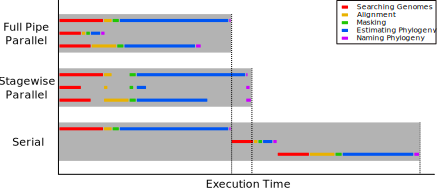
\includegraphics[width=\textwidth]{dd_par.pdf}
    \caption[Tree generation pipeline architectures]{A explanatory plot showing 3 different possible architectures for a tree generation pipeline. 
        Serial, in which each phylogeny is run one after another.  This form makes no use of multiprocessing
        facilities, however, a moderate but significant performance improvement can be achieved by allowing
        each stage in the pipeline to utilise multiple cores i.e. the trees are generated serially but during
        their generation alignment and blasting making use of multiple processors.          
        Stagewise parallel, where for example, all alignments for each input sequence are run side-by-side 
        and masking begins once the last sequence has finished alignment.  The disadvantage of this is a single
        slow stage for one input sequence can hold up the whole pipeline and leave resources idle.  Additionally,
        by running many of the same type of process at the same time, each with similar resource requirements,
        the risk of hardware bottlenecking is increased compared to a more heterogeneous load.
        Finally, fully parallel runs each input sequence through the pipeline stage-by-stage separately
    from all other inputs to the pipeline. This prevents blocking and allows efficient using of resources.}
    \label{fig:ddg}
\end{figure}

40 genomes covering the diversity of the tree of life, with a particular focus on green algal and ciliate representatives 
were selected for this phylogenetic generation: 
\textit{Arabidopsis thaliana}, \textit{Chlamydomonas reinhardtii},
\textit{Ostreococcus tauri}, \textit{Micromonas pusilla CCMP1545},  \textit{Chlorella variabilis NC64A}
\textit{Chlorella vulgaris C-169}, \textit{Physcomitrella patens}, \textit{Saccharomyces cerevisiae S288C}, 
\textit{Neurospora crassa OR74A},
\textit{Homo sapiens},
\textit{Mus musculus},
\textit{Dictyostelium discoideum},
\textit{Paramecium caudatum},
\textit{Paramecium tetraurelia},
\textit{Tetrahymena thermophila macronucleus},
\textit{Oxytricha trifallax},
\textit{Toxoplasma gondii},
\textit{Guillardia theta},
\textit{Bigelowiella natans},
\textit{Emiliania huxleyi CCMP1516},
\textit{Aureococcus anophagefferens},
\textit{Ectocarpus siliculosus},
\textit{Schizosaccharomyces pombe},
\textit{Bacillus cereus ATCC 14579},
\textit{Escherichia coli str. K-12 substr. MG1655},
\textit{Escherichia coli O157 H7 str. Sakai},
\textit{Salmonella enterica subsp. enterica serovar Typhi str. CT18},
\textit{Amycolatopsis mediterranei U32},
\textit{Aquifex aeolicus VF5},
\textit{Borrelia burgdorferi B31},
\textit{Chlamydophila pneumoniae CWL029},
\textit{Chlorobium tepidum TLS},
\textit{Deinococcus radiodurans R2},
\textit{Caulobacter crescentus CB15},
\textit{Sulfolobus islandicus M.14.25},
\textit{Nanoarchaeum equitans Kin4-M},
\textit{Haloferax mediterranei ATCC 33500},
\textit{Methanococcus maripaludis S2},
\textit{Cenarchaeum symbiosum A}.

\subsubsection{Automated Phylogenetic Transcript Binning - Arboretum}
In order to automate phylogeny based transcript binning the 10,000
manually verified phylogenetic bins from the initial BLAST based binning
and analysis were used as a training dataset for supervised classification.

The supervised classification was implemented in a script called ``Arboretum''
The cardinalities of each label in training set was relatively balanced (i.e. all within
the same order of magnitude) 1975 endosymbiont phylogenies, 2600 host, 3456 food, and 1969
unknown. 

``Arboretum'' parses phylogenies and identifies the k (default of 10) nearest branches to the seed transcript
the phylogeny was generated from.  The species of these closest leaves is queried taxonomically using the
NCBI taxonomy local database implemented in the ETE toolkit.  With a set of look-up filters e.g.
sequences from ciliates can be defined as "host-like", a set of vectors is created for each phylogeny.  
These are N-dimensional vectors where N is the number of class labels being used. 
For example, in this specific case: "endosymbiont", "host", "food/bacterial", and "unknown".
The magnitude of each dimension is the summed reciprocal phylogenetic distance between the root node and all
of the nearest branches that have been identified as being indicative of a certain class.
Specifically, if \(\gamma(x,y)\) is the phylogenetic distance between the terminal nodes \(x\) and \(y\), \(\psi(x)\) 
represents the look-up filters and returns the label of the terminal node \(x\) e.g. ``host''.
and \(\delta_{ij}\) is the Kronecker delta\footnote{
    \(\delta_{ij}= \begin{cases}
	1, &  i = j\\
	0, & i \neq j 
	\end{cases} \)}, then for a phylogeny \(A\):
\begin{center}
	\[
X_{A, class} = \sum_{k=1}^K \left( \frac{1}{\gamma(A_k, A_{root})} * \delta_{\psi(A_k),class} \right)
	\]
\end{center}
Where in this specific example ``class'' is one of the set \(\left\{endosymbiont, host, food, unknown\right\}\)
although naturally the classes will be encoded using integer labels.
Therefore, the dimensions of X are \(|A|,|class|\) i.e. the number of training phylogenies by the
number of pre-defined class labels.

Training data was visualised using Radial Visualisation (RadViz) \citep{Hoffman1997,Fayyad2001}.
RadViz is a form of radial co-ordinate visualisation that non-linearly maps a set of N-dimensional 
points onto a plane for easy 2D visualisation. This mapping operates on the physical principle
of ``springs'' anchored evenly around a unit circle with ``spring'' stiffness determined by 
the normalised \(0-1\) value of that dimension for that point.  Each point therefore rests
at the point of mechanical equilibrium between the ``springs'' \citep{NovakovaLenkaandStepankova2006}.

1,000 vectors from this training set were held out to form the test set and all models were then trained
using 5-fold cross-validation (CV) on the remaining 9,000 training vectors. 
We evaluated Support Vector Machines (SVMs) with both linear and radial basis function (RBF) kernels
\citep{Vapnik1963}, naive Bayes, K-neighbours, 
Decision Trees (DT) \citep{Quinlan1986}, DTs ensembles in a Random Forests \citep{Breiman2001}
and Extremely Randomised Trees (ExtraTrees) \citep{Geurts2006},
adaptively boost (AdaBoost) DTs \citep{Freund1997}, Linear Discriminant Analysis (LDA) and
Quadratic Discriminant Analysis (QDA).
Models were trained and hyperparameters were optimised using a randomised search instead of the less
efficient grid search \citep{Bergstra2012} using Bayesian optimisation in the HPOlib library \citep{Eggensperger2013,Komer2014} over the CV-folds.  
Finally, each model was assessed using the held out test set and performance was 
evaluated by inspection of label-wise classification reports containing various
metrics e.g. label F1-scores and confusion matrices.
 
The best performing model and hyperparameters were then used to classify the remaining
unlabelled phylogenies.

\subsubsection{TAXAassign comparison}

To assess the performance of supervised learning and phylogeny based system (Arboretum)
described above a stand-alone sequence identity binning tool TAXAssign (\url{https://github.com/umerijaz/TAXAassign}) was run 
against the 70,605 CDS sequences.  

TAXAssign queried each CDS against the entire NCBI nt database.
The nt BLAST database was downloaded using update\_blastdb.pl script \url{http://www.ncbi.nlm.nih.gov/blast/docs/update_blastdb.pl}
and TAXAssign ran BLASTN in parallel (using GNU parallel \citep{Tange2011a})
with a maximum of 10 reference matches
per CDS a minimum necessary percentage identity for assignment
to a given taxonomic level of 60, 70, 80, 95, 95, and 97
for Phylum, Class, Order, Family, Genus and Species respectively. 

Results were then tabulated and compared with the Dendrogenous-Arboretum assignments.

\section{Results} 

\subsection{Library contamination screening}

Libraries were screened for inclusion in assemblies by inspection of their taxonomic
profiles (see \cref{tab:sct_duey} and \cref{tab:bulk_duey}) as determined by DueyDrop 
and their GC\% probability densities (via KDE).

The GC density estimates of the single cell libraries show a clear bimodal GC density
with a high 70GC\% peak (\cref{fig:gc_prop_raw}) in all dark single cell libraries. 
With the exception of Dark1-2 and Dark2-3 this high GC peak is a greater density
than the expected peak 30-50GC\% (from known GC\% found in genomes
of sequenced relatives of both host and endosymbiont).

\begin{figure}[h!]
    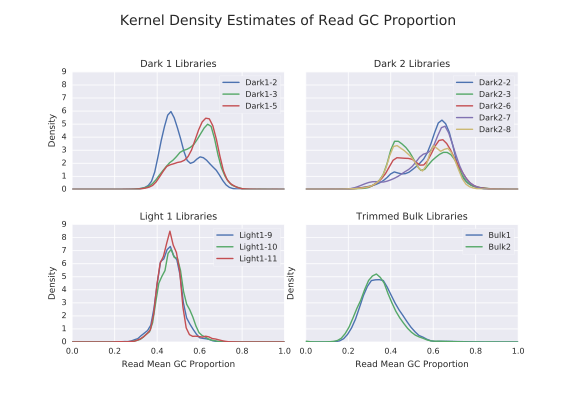
\includegraphics[width=\textwidth]{raw_lib_gc_prop.pdf}
    \caption[GC densities of libraries]{Probability densities of per-read GC proportions for the raw data (apart from pre-trimmed bulk explained previously)
        from each sequenced library.
        Densities were derived using Kernel Density Estimation implemented in Seaborn. 
        Dark 1 (Dark1-2, Dark1-3, and Dark1-5) and Light 1 (Light1-9, Light1-10, Light1-11) 
        were sc-RNAseq from the first round of SCTs sampled during the mid-dark and light 
        culture phases.  Similarly, Dark 2 (Dark2-2, Dark2-3, Dark2-6, Dark2-7, Dark2-8)
        were the libraries sampled in the dark from the second round of SCT.  Bulk1 and Bulk2
        are the bulk RNAseq libraries sequenced under lit and dark conditions. 
        The bulk and single cell light libraries demonstrate similar shaped distributions
        although the bulk has a greater proportion of low GC\% reads potentially representing
        more \textit{Paramecium} derived data. All single cell dark libraries 
        demonstrate a bimodal density with up to the majority of reads deriving 
        from an unknown high 70\% GC population. The dark single cell libraries
        exhibiting a relatively larger peak at 70\% GC than at 40-50\%GC (i.e.
        Dark1-3, Dark1-5, Dark2-2, Dark2-7) were
        the same libraries which were identified as potentially contaminated
        in taxonomic screening (see \cref{tab:sct_duey}).
    }
    \label{fig:gc_prop_raw}
\end{figure}

When these KDE are compared to the densities estimated from the Q20 trimmed
bulk reads (bottom right pane in \cref{fig:gc_prop_raw}) and 
raw bulk RNAseq reads from \citep{Kodama2014} (see \cref{fig:gc_prop_kodama}) 
it is apparent that this high GC\% peak is likely originating from
a high GC\% bacterial contaminant in the Dark single cell libraries.  

One other observation when comparing the bulk RNAseq analyses to the single cell
libraries is that the main GC peak is slightly lower in the bulk (and Kodama dataset), 
around 30GC\% versus 45-50GC\%.
This possibly indicates a greater proportion of reads deriving from the low
GC\% \textit{Paramecium bursaria} host and fewer from the 50GC\% endosymbiont
in bulk libraries relative to single cell libraries.  

\begin{figure}[h!]
	\centering
    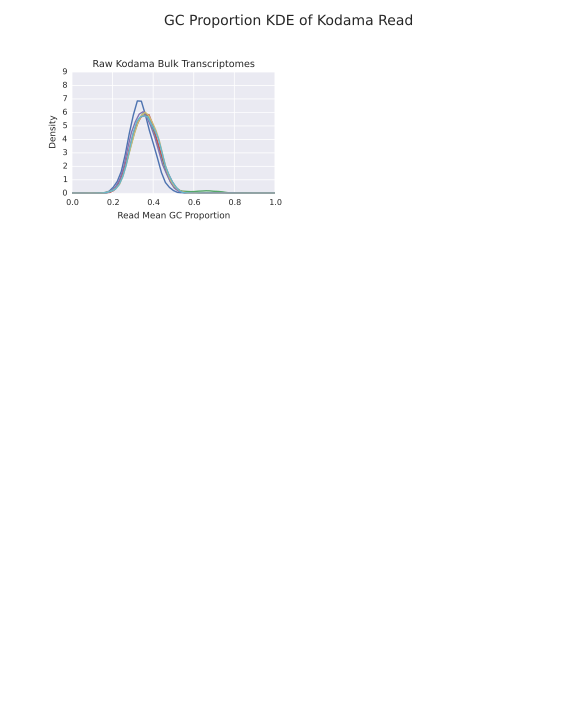
\includegraphics{kodama_gc_prop.pdf}
    \caption[GC densities of \textit{P. bursaria} Yad1g - \textit{C. variabilis} 1N]{Probability density of the per-read GC proportion for 6 raw libraries derived from
        \citep{Kodama2014} transcriptome analysis of a different \textit{P. bursaria} species (Yad1g)
        with and without its \textit{Chlorella variabilis} 1N endosymbiont. Individual libraries are indicated 
        in the key using their DDBJ accession.        
        This dataset displays densities relatively similar
to the bulk RNAseq conducted in this project - ``Trimmed Bulk Libraries'' in \cref{fig:gc_prop_raw}.}
    \label{fig:gc_prop_kodama}
\end{figure}

By comparing the results of the KDE GC analysis with and without read trimming it
is apparent that trimming of reads makes nearly no difference in the density estimates.
The KDE of Q30 sliding window trimmed single cell reads in \cref{fig:gc_prop_q30} is nearly
identical to that of the raw reads \cref{fig:gc_prop_raw}.

\begin{figure}[h!]
    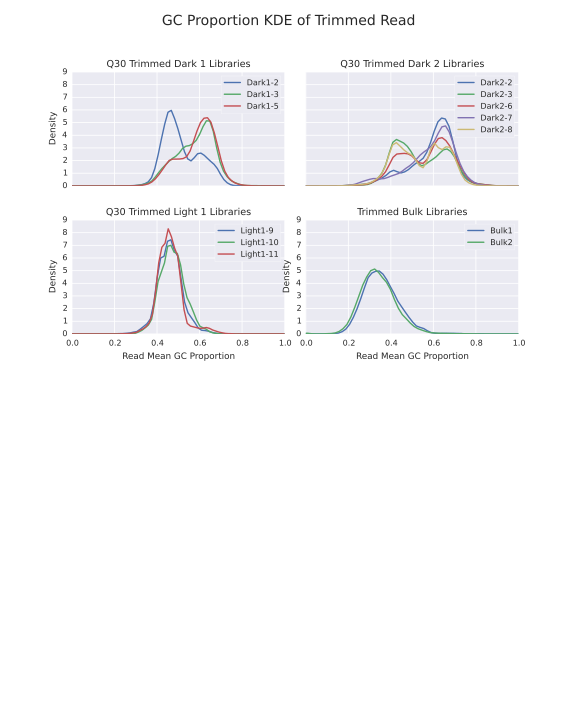
\includegraphics[width=\textwidth]{lib_gc_prop_q30_trimmed.pdf}
    \caption[GC Densities of Bulk Libraries]{Probability densities of per-read GC proportions for trimmed reads.
             To ensure probability densities estimated in \cref{fig:gc_prop_raw}
         weren't biased by low quality ambiguous reads the same analysis was
     repeated using reads trimmed using a sliding window approach with a stringent average
 quality threshold of Q30.  
 In all cases the densities produced appear near identical to
 the analysis of the raw data.}
    \label{fig:gc_prop_q30}
\end{figure}

The taxonomic profiles of single cell (\cref{tab:sct_duey}) and bulk libraries (\cref{tab:bulk_duey}) 
generated by DueyDrop are summarised in the tables below.  It is readily apparent 
that Dark1-3, Dark1-5, Dark2-2, and Dark2-7 display an aberrantly low number of reads
aligning to known alveolate (or even eukaryote) sequences. 
Forward and reverse reads within a library display similar profiles with a slightly
lower proportion of hits in the reverse reads. This can likely be attributed to
the lower read quality found in reverse reads relative to forward reads 
in paired-end Illumina sequencing. 

\begin{table}[h!]
    \resizebox{\textwidth}{!}{\begin{tabular}{|l||l|l|l|l|l|l|l|}
         \hline
         \textbf{SCT Library} & \textit{\textbf{PE}}          & \textbf{Eukaryote} & \textbf{Bacteria} & \textbf{Alveolate} & \textbf{Viridiplantae} &  & \textbf{Total Hits} \\ 
         \hline
         \textit{Light1-9}    & \textit{R1}                   & 51.89 +/- 0.45     & 9.37 +/- 0.26     & 25.15 +/-  0.71    & 7.45 +/- 0.33          &  & 69.49 +/- 0.37      \\ 
                              & \textit{R2}                   & 51.75 +/- 0.25     & 8.82 +/- 0.24     & 24.85 +/- 0.56     & 7.49 +/- 0.21          &  & 68.75 +/- 0.29      \\ 
         \textit{Light1-10}   & \textit{R1}                   & 46.35 +/- 0.56     & 15.72 +/- 0.46    & 22.96 +/- 0.24     & 6.94 +/- 0.26          &  & 68.73 +/- 0.30      \\ 
                              & \textit{R2}                   & 46.12 +/- 0.83     & 15.14 +/- 0.48    & 23.13 +/- 0.38     & 6.99 +/- 0.37          &  & 68.73 +/- 0.30      \\
         \textit{Light1-11}   & \textit{R1}                   & 58.28 +/- 0.47     & 3.62 +/- 0.12     & 28.68 +/- 0.43     & 8.20 +/- 0.40          &  & 71.38 +/- 0.49      \\ 
                              & \textit{R2}                   & 57.74 +/- 0.27     & 3.50 +/- 0.10     & 28.23 +/- 0.36     & 8.41 +/- 0.31          &  & 70.42 +/- 0.20      \\
         \textit{Dark1-2}     & \textit{R1}                   & 28.64 +/- 0.51     & 22.88 +/- 0.61    & 12.23 +/- 0.28     & 4.93 +/- 0.19          &  & 60.31 +/- 0.49      \\ 
                              & \textit{R2}                   & 28.29 +/- 0.24     & 21.06 +/- 0.21    & 12.13 +/- 0.28     & 4.87 +/- 0.34          &  & 57.65 +/- 0.35      \\
         \textbf{\textit{Dark1-3}}     & \textit{R1}          & 9.48 +/- 0.43      & 25.07 +/- 0.42    & 2.15 +/- 0.13      & 2.60 +/- 0.27          &  & 41.43 +/- 0.68      \\ 
                              & \textit{R2}                   & 8.89 +/- 0.19      & 23.11 +/- 0.52    & 2.13 +/- 0.16      & 2.45 +/- 0.18          &  & 38.50 +/- 0.46      \\
         \textbf{\textit{Dark1-5}}     & \textit{R1}          & 5.56 +/- 0.19      & 23.99 +/- 0.44    & 1.07 +/- 0.07      & 2.89 +/- 0.11          &  & 36.72 +/- 0.33      \\ 
                              & \textit{R2}                   & 4.94 +/- 0.21      & 21.75 +/- 0.53    & 1.02 +/- 0.11      & 2.33 +/- 0.17          &  & 33.06 +/- 0.52      \\
         \textbf{\textit{Dark2-2}}     & \textit{R1}          & 12.32 +/- 0.25     & 9.81 +/- 0.19     & 3.73 +/- 0.16      & 4.33 +/- 0.17          &  & 27.65 +/- 0.47      \\ 
                              & \textit{R2}                   & 11.53 +/- 0.15     & 9.00 +/- 0.17     & 3.67 +/- 0.22      & 3.74 +/- 0.12          &  & 25.71 +/- 0.39      \\
         \textit{Dark2-3}     & \textit{R1}                   & 32.07 +/- 0.31     & 7.43 +/- 0.15     & 12.81 +/- 0.21     & 4.71 +/- 0.21          &  & 48.42 +/- 0.53      \\ 
                              & \textit{R2}                   & 32.47 +/- 0.24     & 6.68 +/- 0.21     & 13.11 +/- 0.43     & 4.58 +/- 0.12          &  & 47.92 +/- 0.28      \\
         \textit{Dark2-6}     & \textit{R1}                   & 24.11 +/- 0.28     & 8.55 +/- 0.11     & 9.04 +/- 0.35      & 5.27 +/- 0.15          &  & 41.69 +/- 0.45      \\ 
                              & \textit{R2}                   & 22.89 +/- 0.55     & 7.44 +/- 0.17     & 8.74 +/- 0.49      & 4.36 +/- 0.24          &  & 38.85 +/- 0.58      \\
         \textbf{\textit{Dark2-7}}     & \textit{R1}          & 9.96 +/- 0.24      & 16.89 +/- 0.27    & 4.22 +/- 0.24      & 2.83 +/- 0.17          &  & 37.06 +/- 0.40      \\ 
                              & \textit{R2}                   & 8.77 +/- 0.18      & 15.00 +/- 0.43    & 3.94 +/- 0.14      & 2.16 +/- 0.11          &  & 32.86 +/- 0.29      \\
         \textit{Dark2-8}     & \textit{R1}                   & 28.24 +/- 0.48     & 4.45 +/- 0.13     & 12.00 +/- 0.32     & 4.69 +/- 0.06          &  & 40.50 +/- 0.37      \\ 
                              & \textit{R2}                   & 28.22 +/- 0.47     & 4.30 +/- 0.22     & 11.98 +/- 0.37     & 4.32 +/- 0.24          &  & 40.05 +/- 0.22      \\
         \hline
 \end{tabular}}
     \caption[DueyDrop Taxonomic Profile Summary]{Taxonomic profiles of raw single cell libraries generated using ``DueyDrop''. All values are percentage of reads mapping to that category +/- the standard deviation between sample replicates.  
         The analysis was conducted for both forward and reverse reads from each library (indicated as R1 and R2 in the paired-end (PE) column).
         Libraries highlighted in bold were those excluded from subsequent analysis on the basis of their very low numbers of reads identifiable as 
 eukaryotic (or specifically alveolate or archaeplastida). All forward and reverse read pairs display similar profiles to one another suggesting
 the problem of ``MDA chimeras'' may be minor.}
 \label{tab:sct_duey}
\end{table}

The bulk libraries demonstrate a very low level of hits compared to single cell libraries (see \cref{tab:bulk_duey}), 
to the point where if they were single cell libraries they would be taxonomically excluded. 
However, it should be noted that the bulk libraries were sequenced on a Gene Analyzer II and are on average
half the length of single cell reads (76bp vs 150bp). Due to the difficulty aligning short reads
to references the difference between libraries may be attributable to this alone. 
Additionally, the vast majority of the lower number of hits do align to eukaryote (and alveolate) 
taxa consistent with an non-contaminated library. 

\begin{table}[h!]
     \begin{tabular}{|l|l|l|l|l|l||l|}
\hline
         \textbf{Bulk Library} & \textit{\textbf{PE}} & \textbf{Eukaryote} & \textbf{Bacteria} & \textbf{Alveolate} & \textbf{Viridiplantae} &  \textbf{Total Hits} \\ 
         \hline
         \textit{Light}    & \textit{R1}              &  9.66 +/- 1.55     & 0.18 +/- 0.13     &  6.28 +/- 1.41     &  0.86 +/- 0.3          & 10.10 +/- 1.48       \\
                              & \textit{R2}           &  9.62 +/- 0.81     & 0.26 +/- 0.09    &  6.58 +/- 0.36     &  1.04 +/- 0.41         &   10.16 +/- 0.95      \\ 
                              \hline 
         \textit{Dark}   & \textit{R1}                &  4.90 +/- 0.78     & 0.36 +/- 0.11    &  3.14 +/- 0.58     &  0.50 +/- 0.16        &   5.40 +/- 0.93      \\ 
                              & \textit{R2}           &  5.50 +/- 1.25     & 0.22 +/- 0.19   &  3.82 +/- 0.81     &  0.50 +/- 0.12         &  6.02 +/- 1.22      \\ 
                              \hline
    \end{tabular}
    \caption[Taxonomic Profiles of Bulk Libraries]{Taxonomic profile of the two trimmed (Q20) bulk transcriptome libraries generated using ``DueyDrop''.
All values are the percentage of reads mapping to that taxonomic category +/- the standard deviation between sampling replicates.  
The analysis was conducted for both forward and reverse reads from each library (indicated as R1 and R2 in the paired-end (PE) column).
Overall only a very small number of bulk reads could be assigned to any taxonomic class by ``DueyDrop''.}
    \label{tab:bulk_duey}
\end{table}

To identify the likely source of the high GC\% contamination 
and to assess how representative the taxonomic profiling of small random
subsamples of reads \(\leq1\%\) to full scale analyses Krona was used to 
create interactive hierarchical plots of the taxonomic profiles\footnote{
Accessible at \url{http://finlaymagui.re/dueydrop_analysis}} 
From this, Rhizobia species are the most prevalent high GC\% species found in the libraries
with this high 70GC\% peak in the KDE plots and therefore are the most likely source
of this particular aspect of contamination. 

\begin{figure}[h!]
    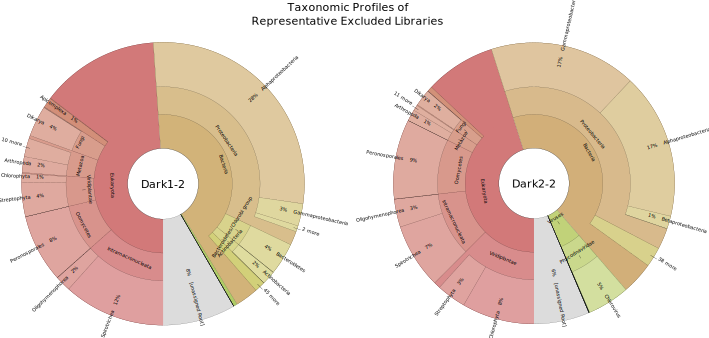
\includegraphics[width=\textwidth]{krona_excluded_raw.pdf}
    \caption[Visualisation of taxonomically excluded libraries]{Krona visualisation of taxonomic profiles of two representative
        single cell libraries (Dark1-2, Dark2-2) that were excluded from further analysis due 
    to aberrant profiles (typically large proportion of reads being assigned
    to Bacteria than Eukaryota). Note that nearly \(50\%\) of each library is identified as bacterial.}
    \label{fig:krona_excluded}
\end{figure}

\begin{figure}[h!]
    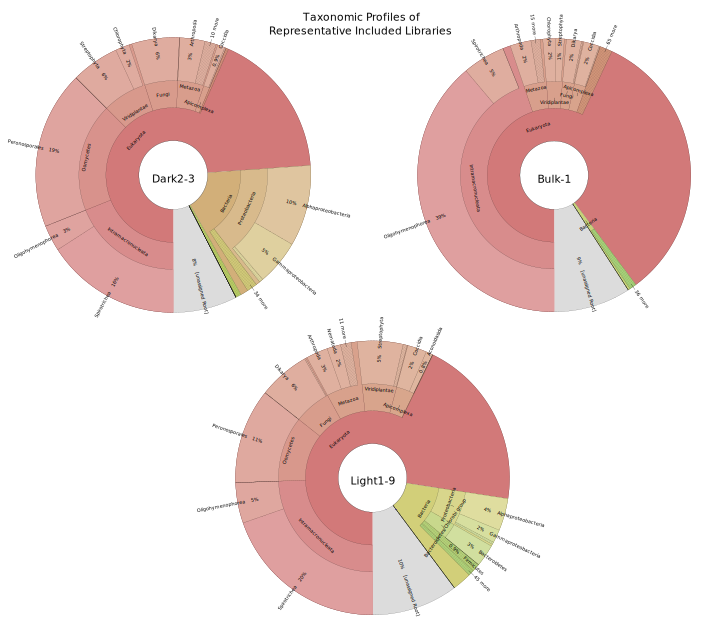
\includegraphics[width=\textwidth]{krona_included_raw.pdf}
    \caption[Visualisation of taxonomically included libraries]{
    Krona visualisation of the taxonomic profiles of representative 
    RNAseq libraries (Bulk1, Dark2-3, and Light1-9) that were retained 
    in the analysis after taxonomic screening.  The key thing this figure
    shows is that in retained libraries the vast majority of reads were 
    identified as eukaryotic in origin.
    }
    \label{fig:krona_included}
\end{figure}


\begin{figure}[hp]
    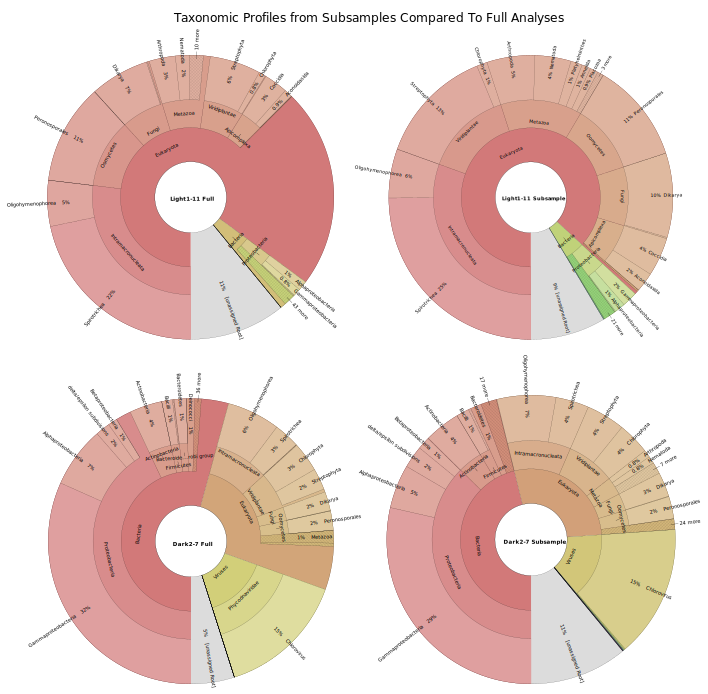
\includegraphics[width=\textwidth]{krona_all_vs_sample.pdf}
    \caption[Comparison of Subsample to Whole Library Profiles]{Comparison of taxonomic profiles derived from small \(\leq1\%\)
        random subsamples of libraries compared to profiles generated using the
        full library.  Light1-11 and Dark2-5 are used as representative examples
        as they display the trends common for all single cell libraries. 
        All subsamples demonstrated taxonomic profiles with relatively similar
        proportions to full analyses.  For example, in the Light1-11 subsample
        of reads with hits the proportion of eukaryote to Bacteria was 87:4 
        \% vs 85:4\% of the root for the full analysis. Similarly the ratios
        for Dark2-7 shown eukaryote to bacteria are 26:54 for full analysis
        and 28:46 for subsample. 
        The key difference is the assignment of a greater proportion of reads to 
        intermediate taxonomic levels in the full analyses due to the difference in 
        resolution of multiple hits per read.  Principally, the full library analyses
        retain all hits and assign level based on a lowest common ancestor algorithm
        whereas the subsample analysis just uses the top hit.
    }
    \label{fig:krona_sample_vs_full}
\end{figure}

Therefore, small random subsamples are representative of the full library and
read-level taxonomic assignment can be used to screen single cell libraries for contamination.


\subsection{Read pre-processing} 

\subsubsection{Trimming optimisation}

The optimal trimming threshold was determined by a combination
of read mapping statistics against 3 preliminary reference assemblies
as well as the impact on resultant \textit{de novo} assemblies at 
that threshold.

A rapid decrease in the number of concordantly mapping PE reads (i.e.
within insert distance of one another) was observed above a Q30 quality threshold.
This proves true regardless of the reference assembly being mapped to
(see \cref{fig:trimmingopt}).  Q30 relative to Q20 appears to induce a 
very slight decrease in total number of mapping reads but not drastically so. 

\begin{figure}[hp]
	\centering
    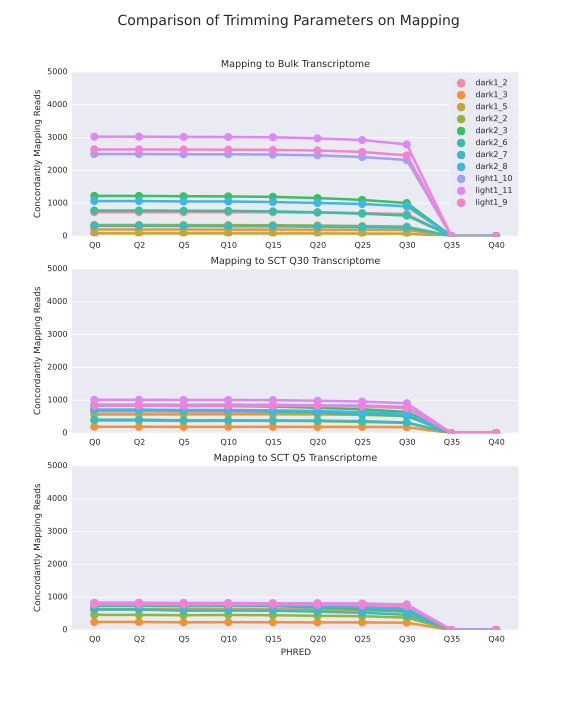
\includegraphics[width=0.9\textwidth]{trimmingopt.pdf}
    \caption[Optimising trimming thresholds]{Assessment of the optimal minimum average quality threshold
             in Trimmomatic's sliding window (size 4) trim.  Plots
             display the number of concordantly mapping reads (i.e. the forward
                 and reverse read map to assembly at a distance of approximately
                 their insert)
             at a range of different trimming
             thresholds.  5000 randomly sampled PE reads 
             from each single cell library are mapped against 3 different 
             reference assemblies. 
             The key finding is above a threshold of Q30 there is a huge
         decrease in the number of mapping reads.}
         \label{fig:trimmingopt}
\end{figure}

Additionally, naive assemblies in Trinity of taxonomically screened single cell libraries
at different sliding window quality threshold trims of Q5, Q20, and Q30 (\cref{tab:trim_assembly})
were created. 
These show that more permissive trims (Q5 and Q20) lead to a greater number of assembled bases and transcripts 
however the likelihood of these assemblies are also lower than that generated using the 
more conservative Q30 trim. 
However, it should be noted that the difference in the number and size of assembled transcripts at different thresholds 
was less than was found using different assemblers and assembly parameters.

\begin{table}[h!]
    \centering
    \begin{tabular}{|l| l |l |l|}
     	\hline
         \textbf{Trim Threshold} & \textbf{Number of Transcripts} & \textbf{Bases Assembled} & \textbf{Assembly Likelihood (\(-\log\))} \\
         \hline
         Q5 &  112,182 & 52,511,552 & \(-3.168*10^{10}\) \\
         Q20 & 107,955 & 50,809,686 & \(-3.015*10^{10}\) \\
         Q30 & 99,784 & 47,313,963 &  \(-2.832*10^{10}\) \\ 
    \hline
\end{tabular}
    \caption[Comparison of Effect of Trimming on Trinity Assemblies]{Comparison of Trinity assemblies of taxonomically screened
        single cells reads (no bulk reads) at 3 different sliding window
        minimum average quality trimming thresholds.  Trimming largely
        does not cause a major difference between assemblies in terms of number
        of contigs recovered or overall assembly likelihoods.  Harsher (Q30) trims 
        result in slightly smaller but slightly more likely assemblies than permissive
        trims (Q5).
    }
    \label{tab:trim_assembly}
\end{table}

Therefore, due to increasing the assembly likelihood while only very marginally
decreasing the number of contigs and mapping reads relative to
more permissive trims Q30 was determined to be the optimal trimming threshold.
It can be considered from this data that Q30 forms a maximum feasible stringency for trimming. 

\begin{table}
    \centering
    \begin{tabular}{|r||l|l|}
        \hline
        \textbf{Library} & \textbf{Number of raw PE Reads} & \textbf{Number of Q30 trimmed PE Reads} \\
        \hline
        Dark1-2 &  \(6.460*10^{7}\) &  \(3.355*10^{6}\)\\ 
        Dark2-3 & \(2.243*10^7\)&  \(1.478*10^7\)\\
        Dark2-6 & \(2.431*10^7\) & \(1.443*10^7\) \\
        Dark2-8 & \(2.761*10^7\) &  \(1.866*10^7\) \\
        Light1-9 & \(1.524*10^7\) & \(1.382*10^7\) \\
        Light1-10 & \(1.614*10^7\) & \(1.478*10^7\) \\
        Light1-11 & \(1.474*10^7\) & \(1.334*10^7\) \\
        \hline
    \end{tabular}
    \caption[Library Sizes After Trimming]{Summary of the library size of the taxonomically selected single cell 
        libraries before and after trimming at a minimum average SLIDINGWINDOW quality 
        threshold of Q30. Of interest, Dark1-2 was generally of poor quality and thus 
        was disproportionately minimised by trimming. Additionally, the 
        two bulk RNAseq libraries were trimmed at Q20 in FastQ-MCF resulting in 
    total library sizes of \(2.458*10^{7}\) and \(2.779*10^{7}\) respectively}
\end{table}

\subsubsection{GC partitioning} 

GC partitioning was conducted on Q30 trimmed reads 
using K-means clustering as implemented in the parKour tool described above 
to attempt to remove GC\% rich contamination from single cell libraries.

The 2 different clustering schemes attempted using 2 and 3 target clusters.
Additionally, both clustering schemes were also run with an initial overclustering factor of 3
i.e. parKour originally found 6 and 12 clusters and then merged them to produce the target 2 and 3 
clusters respectively. 

\begin{table}
    \centering
    \begin{tabular}{|c||c|c|}
        \hline
        \textbf{Clustering Scheme} & \textbf{Centroids} & \textbf{Number of Reads Assigned} \\
        \hline
        2                    & (0.6674, 0.6177) & 57.3M \\
                             & (0.4557, 0.4393) & 81.6M \\
        \hline
        2 (over-clustering)   & (0.6672, 0.6168) & 57.7M \\
                             & (0.4555, 0.4392) & 81.2M \\
        \hline
        3                    & (0.5363, 0.5092) & 44.0M \\
                             & (0.6924, 0.6394) & 43.3M \\
                             & (0.4231, 0.4096) & 51.6M \\
        \hline
        3 (over-clustering)   & (0.5365, 0.5090) & 43.9M \\
                             & (0.6921, 0.6396) & 43.6M \\
                             & (0.4235, 0.4098) & 51.7M \\
        \hline
    \end{tabular} 
    \caption[ParKour Cluster Summaries]{Final cluster centroids and number of reads assigned
    to each cluster in parKour using various run settings.  Centroids
    are the mid-point of each cluster, therefore in the 2 cluster scheme
    ``parKour'' identified one cluster of reads centred around  
    \(66.74\%\) GC for the forward read and \(61.77\%\) for the reverse read.
    Note that 
    overclustering made a minimal impact on cluster location.}
    \label{tab:centroids} 
\end{table} 

2 and 3 target clusters with and without an initial 
overclustering factor of 3 (i.e. initially finding 6 and 12 clusters originally before merging to
produce final 2 and 3 cluster targets). 

Therefore, over-clustering made a minimal effect on cluster centroids and read assignment.

\begin{figure}[h!]
	\centering
    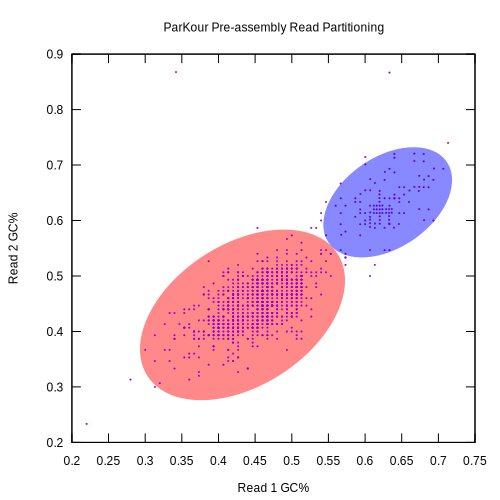
\includegraphics[width=0.9\textwidth]{parKour.pdf}
    \caption[Plot of parKour clusters]{Visualisation of GC-based paired read K-means clustering on a small random subset of all single cell transcriptome
        reads. 2 initial centroids were specified without an overclustering factor and approximate final centroids (0.6674, 06177) and (0.4557, 0.4393) are indicated by highlighted areas.  57.3M and 81.7M were assigned to each respective cluster. Comparison to other clustering regimes can be found in \cref{tab:centroids}.  This supports the finding of the \cref{fig:gc_prop_raw}that there is a clear and identifiable cluster of high GC\% reads present in the sample and it is possible to identify and group these reads using unsupervised learning. 
} 
        \label{fig:parkour} 
\end{figure}

Unfortunately, as might have been foreseen, the resultant assemblies from individual
read clusters displayed high levels of fragmentation regardless of the clustering
regime used.  For example, in the case of the 2 cluster (without over-clustering) 
and subsequent individual Trinity-based assemblies resulted in 268,806 transcripts
of marginally shorter average length than the equivalent un-pre-partitioned assembly
(99,784 transcripts).

The same pattern, consistent with assembly fragmentation, 
was observed when only dark single cell libraries were clustered using 
2 or 3 clusters. 
Therefore, GC-based pre-assembly read partitioning proved incapable of improving
the assembly of this highly heterogeneous RNAseq dataset.


\subsubsection{Error correction}

Error correction was attempted on both lightly trimmed (Q5) and harshly trimmed (Q30) 
taxonomically selected SCT reads.

Bayeshammer, as implemented in the Spades genome assembler, even on permissively trimmed
(\(Q>5\)) reads corrected only a maximum \(0.0007\%\) of reads in the 7 taxonomically selected SCT libraries.
As this affected on the order of 10s of reads it was not considered worth pursuing this tool further.

``SEECER'', an RNA-Seq specific error correction tool was used to correct 
lightly trimmed (Q5) and harshly trimmed (Q30) SCT reads.  
Approximately, \(5.37\%\) of Q5 trimmed SCT reads
were corrected in ``SEECER''. \(0.51\%\) of Q30 trimmed
SCT reads were corrected.  

Trinity assemblies of taxonomically selected single cell libraries 
(without bulk libraries) were then compared with and without ``SEECER'' 
error correction (see \cref{tab:errcorr_assembly}).
\begin{table}[h!]
    \begin{tabular}{|l||r|r|l|@{}}
     	\hline 
         \textbf{Trim Threshold} & \textbf{Number of Transcripts} & \textbf{Bases Assembled} & \textbf{Assembly Likelihood (\(-\log\))} \\
         \hline 
         Q5 &  112,182 & 52,511,552 & \(-3.168 \cdot 10^{10}\) \\
         Q5 SEECER Corrected & 111,853 &  51,847,128 & \(-3.147\cdot 10^{10}\) \\
         Q30 & 99,784 & 47,313,963 & \(-2.912\cdot 10^{10}\)  \\ 
         Q30 SEECER Corrected & 96,494 & 46,312,469 & \(-2.995\cdot 10^{10}\)  \\ 
    \hline
\end{tabular}
    \caption[Effect of Error Correction on Assembly]{Naive Trinity assembly of Q5 and Q30 trimmed taxonomically selected single cell libraries
        with and without SEECER error correction. While assembly likelihood increases after
    error correction for Q5 trimmed reads it is still lower than Q30 uncorrected.  For Q30
trimmed reads error correction marginally decreases assembly likelihood.}
    \label{tab:errcorr_assembly}
\end{table}

As can be observed, error correction of SCT reads made minimal effect in the overall likelihood
of assemblies for this dataset even with lightly trimmed reads.  Error corrected Q5
trimmed reads performed worse than Q30 trimmed reads without error correction. 
Additionally, Q30 trimmed reads generated marginally less likely assemblies with 
error correction than without. 

Therefore, error correction
was considered ineffective for this dataset and thus was not used 
used for further analysis.  Instead, we elected to use uncorrected, taxonomically selected,
Q30 trimmed reads from this point on. 

\subsubsection{Digital Normalisation} 
Digital normalisation and removal of likely erroneous k-mers (i.e. low abundance) 
via Khmer reduced the total input reads from the Q30 trimmed taxonomically
filtered SCT and bulk libraries from 
\(2.912\cdot 10^{8}\) to \(8.473\cdot 10^6\) paired reads.

Of those, \(6,231\cdot 10^{6}\) derive from the bulk and \(2.253\cdot 10^6\) 
from single cell libraries. 
Therefore, as Q30 trimmed single cell libraries comprised
\(9.318\cdot 10^{6}\) paired end reads and bulk libraries 
consisted of \(52.377\cdot 10^6\) reads digital normalisation
and abundance filtering resulted in a retention of 
\(2.418\%\) of single cell PE reads and \(11.891\%\) of
bulk PE reads.

Of these surviving single cell PE reads \(9.762*10^{5}\) 
were from the 3 selected light libraries (Light1-9, Light1-10, and Light1-11) 
and \(1.277*10^{6}\) were derived from the dark libraries (Dark1-2, Dark2-3,
Dark2-6, and Dark2-8).  Therefore, abundancy filtering and digital normalisation
did not disproportionately remove light or dark single cell reads.

This Khmer based pre-processing had a very positive effect on 
assembly likelihoods.  The standard Trinity assembly improved in
likelihood by an order of magnitude 
while assembling more transcripts of near equal length (based on
median contig length).  The Khmer processed assembly marginally increased
median contig length at the expense of a lower N50. 

\begin{table}[h!]
    \centering
    \begin{tabular}{|l||r|r|r|r|c|}
     	\hline
        \textbf{Preprocessing} & \textbf{Number of} & \textbf{Bases} & \textbf{Contig} & \textbf{Median} & \textbf{Assembly} \\
                                & \textbf{Transcripts} & \textbf{Assembled} & \textbf{N50} & \textbf{Contig} & \textbf{Likelihood (\(-\log\))} \\
         \hline
         Q30 and Bulk &  127,508 & 83,264,944 & 851 & 411 & \(-2.832 \cdot 10^{10}\) \\
         \hline
         Q30 and Bulk  & 147,902 & 92,395,841 & 789 & 423 & \(-1.224 \cdot 10^{9}\) \\  
    with Khmer & 	 & 			 &      & 	  & 	\\
    processing & 	 & 			 &      & 	  & 	\\
    \hline
\end{tabular}
    \caption[Effect of Digital Normalisation on Assembly]{Trinity assemblies (with --min-kmer-cov 2) 
        of Q30 trimmed, taxonomically selected single cell and bulk libraries 
    with and without Khmer digital normalisation and K-mer abundance filtering.
    Khmer pre-processing improved the assembly likelihood by an order of magnitude,
    and significantly increased the total size of the assembly while only having
    a marginally negative effect on contig N50s. 
    }
    \label{tab:diginorm_assembly}
\end{table}

As Khmer pre-processing both significantly improved assembly run time as well as the overall
assembly quality (as assessed in the Trinity assembly comparison metrics above \cref{tab:diginorm_assembly})
digitally normalised and K-mer abundance filtered bulk and taxonomically selected Q30
trimmed SCT were determined to be the optimal pre-processing for this dataset. 

\subsection{Assembly}

\subsubsection{Referenced}

Referenced assembly using the divergent \textit{Chlorella NC64A},
\textit{Coccomyxa subellipsoidea} C-169, \textit{Tetrahymena thermophila},
\textit{Paramecium caudatum} genomes as references was largely ineffectual.
Of all bulk and SCT reads only \(0.3\) and \(0.4\%\) mapped to the 
algal references respectively.  Similarly, only \(0.6\) and \(0.9\%\) of reads mapped 
to the related ciliate genomes.   This level of mapping is on the order
of random chance. Of the read which mapped, a high proportion (\(73-82\%\))
mapped non-uniquely. 
This suggests mapping was occurring in low complexity regions and is a statistical
artefact for the most part instead of biological significance.

The addition of gene junction annotation files for the reference genomes to improve
spliced mapping only improved the percentage of reads mapping by \(0.05-0.3\) percentage points.  
With so few reads mapping, any attempt to class transcripts from this using cufflinks 
resulted in \(10-23\) total transcripts.

Therefore, referenced assembly using divergent related genomes proved impossible
for this dataset.

\subsubsection{\textit{de novo} assembly} 

The results of the initial assembler comparison using the Q30 trimmed
taxonomically selected SCT libraries (Light1-9, Light1-10, Light1-11, 
Dark1-2, Dark2-3, Dark2-6, Dark2-8) and bulk libraries are shown in
\cref{tab:assemblies}. 

\begin{table}[h!]
    \centering
    \begin{tabular}{|l||c|r|c|c||}
        \hline
        \textbf{Assembler} & \textbf{Parameters} & \textbf{Number of} & \textbf{Bases Assembled} & \textbf{Assembly} \\
          &   & \textbf{Contigs}										& 							& \textbf{Likelihood \(-\log\)} \\
        \hline
        \hline
        SOAPdenovo-Trans & K23 & 374,325 & \(7.64\cdot10^{7}\) & \(3.778\cdot10^{10}\) \\
                         & *K64 & - & - & - \\  
                       & *K80 & - & - & - \\ 
        \hline
        TransAbyss & K20 & 3,272,137 & \(1.722\cdot10^{8}\)   & -  \\
                   & K32 & 853,079   & \( 1.321\cdot 10^{8}\)  & -  \\
                   & K64 & 376,280   & \( 9.755\cdot 10^{7}\)  & -  \\
                   & Merged & 3,055,851 & \(2.71\cdot10^{8}\) & \(-3.113\cdot 10^{10}\)  \\
        \hline
        Oases*     & - & - & - & - \\
        \hline
        IDBA-tran      & - & 54,113 & \(2.7\cdot 10^{7}\) & \(-4.589\cdot 10^{10}\)\\
        \hline
        IDBA-MTP/UD/MT** & - & - & - & \\
        \hline
        Trinity & min\_kmer\_cov 2 & 127,508 &  \( 8.326\cdot 10^{7}\) & \(-2.832\cdot 10^{10}\) \\
        \hline
        Bridger & K25 & 114,582 & \( 9.707\cdot 10^{7}\)  & \(-2.587\cdot 10^{10}\)\\ 
        \hline
        
    \end{tabular}
    \caption[Summary of Different Assembler Outputs]{\textit{De novo} assemblies of Q30 trimmed taxonomically
        selected single cell libraries and bulk libraries (but not digitally normalised or K-mer abundance
            filtered) with a range of assemblers and parameters.  K-mer size used
            for assemblers with that option are indicated in the Parameters column 
            e.g. K23 indicates a 23-mers. Bridger and Trinity outperformed 
            other assemblers in terms of assembly likelihood and rational
            contig numbers and sizes.
        * indicates assemblies programs that failed to run to completion due to 
        insufficient computational resources (despite using a server with 500GB 
        of memory)
        ** indicates assemblies which failed due to coding errors in the application.}
        \label{tab:assemblies}
\end{table}

Critically, Oases, the IDA-MTP/UD/MT pipeline and SOAPdenovo-Trans at higher K-mer values
all failed to run to completion correctly with the dataset.  In the case of Oases
and SOAPdenovo-Trans at higher K-mer values this was due to exhaustion
of system memory and in the case of IDBA-MTP/UD/MT workflow an unresolved coding error 
resulting in repeated segmentation faults.

However, Trinity and Bridger both consistently generated assemblies of approximately
equal size (100-130,000 contigs of rational sizes: N50s of 700-850
    and mean and median contig sizes of 600-660 and 410-470) across a variety 
    of assembly parameters (not shown).  Furthermore, they both consistently
    generated the assemblies with the greatest likelihoods (from RSEM-Eval), 
    and ran most computationally efficiently. 


Trinity and Bridger assemblies using digitally normalised and K-mer abundance 
filtered, taxonomically selected, Q30 trimmed, single cell and bulk libraries performed 
even better in terms of assembly likelihood and read incorporation.

\begin{table}[h!]
    \begin{tabular}{|l|r| r| r| r|}
    	\hline
        \textbf{Assembler} & \textbf{Parameters} & \textbf{Contigs} & \textbf{Bases Assembled} & \textbf{Assembly Likelihood (\(-\log\))} \\
        \hline
        Bridger & K19 & 102,686 & \(8,209*10^{7}\)  & \(-1.729*10^{9}\) \\
                & K25 & 113,106 & \(9.866*10^{7}\)  & \(-1.183*10^{9} \) \\ 
                & K31 & 112,391 & \(8.941*10^{7}\)  & \(-1.143*10^9\) \\ 
        Trinity & Minimum K-mer Coverage of 1 & 176,097 &  \(1.113*10^{8}\)& \(-1.214*10^{9}\) \\  
                & Minimum K-mer Coverage of 2 & 147,902 & \(9.239*10^{7}\) & \(-1.238*10^9\) \\  
                \hline
    \end{tabular}
    \caption[Trinity vs. Bridger Assemblies]{Assembly summaries of Q30 trimmed taxonomically selected SCT and bulk reads 
    after digital normalisation and K-mer abundance filtering. Parameters used in the assembly
indicates any special parameter settings used in the assembly i.e. K19 indicates a K-mer size of 19 was used.
}
    \label{tab:digassemby}
\end{table}

Smaller K-mer values (19-mer) performed worse in the case of the Bridger assembly
with the optimal assembly in terms of contig number and size was the K-mer size 
of 25.  This was slightly lower in terms of likelihood than the 31-mer Bridger
assembly. The digitally normalised and filtered Trinity assemblies 
generated much larger assemblies overall but still produced good likelihoods.

\subsubsection{Assembly combination}

Two assemblies were combined using the tr2aacds.pl script in EvidentialGene 
and a minimum CDS size of 100. The first consisted of all successfully completed
assemblies of non-normalised/filtered reads i.e. SOAPdenovo-Trans, TransAbyss (multiple K-mer
assembly merged using built-in tool),
IDBA-tran, Trinity and Bridger in \cref{tab:assemblies}.  The second, 
of the 3 Bridger digitally normalised assemblies and two Trinity assemblies 
described in \cref{tab:digassemby}.

\begin{table}[h!]
    \begin{tabular}{|r ||r |r | l| }
    	\hline 
        \textbf{Assembly} & \textbf{Input Contigs} & \textbf{Collapsed Contigs} & \textbf{Assembly Likelihood (\(-\log\))}\\ 
        \hline
        Non-normalised Assemblies   & 3,726,379 & 46,063  & \(-4.347*10^{10}\) \\
        Normalised Assemblies       & 652,182 & 53,628 & \(-1.823*10^{9}\)\\
        \hline 
        \textbf{CD-HIT \(90\%\) meta-clustering} & 99,691 & 94,628 & \(-5.133*10^{10}\)\\
        \hline
    \end{tabular}
    \caption[Merged Assembly Summary]{Summary of merged multi-assemblies.  Collapsed contigs is the number of contigs
    found in the merged set by the EvidentialGene pipeline. The level of assembly
reduction and redundancy removal is high and, at first appearance, is impressively consistent 
between meta-assemblies despite differences in preprocessing. 
  However, CD-HIT metaclustering
at 90\% identity shown at the bottom demonstrated that there was very little overlap between
these two minimised assemblies.  Even the merged normalised assemblies generated
a meta-assembly of lower overall likelihood than the best individual constituent assemblies.}
    \label{tab:comb_assemb}
\end{table}

The combination of all non-normalised assemblies produced a surprisingly small
set of contigs, however, also both assemblies also had lower likelihoods than 
any of their constituent assemblies. It is of interest that despite both
generating similar numbers of contigs there was next to no overlap between 
the two combinations as assessed by clustering using CD-HIT at a similarity of \(90\%\).

Therefore, the assembly selected for downstream binning and analysis was Bridger 
assembly of bulk and library screened single cell normalised and K-mer
abundancy filtered reads with a K-mer size of 31 as it displayed the best likelihood
while maintaining assembly statistics within expected ranges. 


\subsection{Binning}

\subsubsection{ORF calling}

From the 112,391 contigs in the final selected assembly (31-mer Bridger
Normalised and Taxonomically Selected SCT and Bulk) - 1,005,370 ORFs
longer than 30 amino acids were identified using a ``Tetrahymena'' encoding.
Using the 500 longest of these ORFs to train a Markov Model and removing
shorter ORFs that lay entirely within a longer ORF resulted in a final set
of 70,605 ORFs.

\subsubsection{Performance of BLAST-based binning}
\(10,000\) of these ORFs were randomly selected and used to search the NCBI
nr database with BLASTP with an expectation of \(1e-5\).  Based on the taxonomic
provenance of the top-hit these ORFs were assigned to a particular originating
bin.  
The initial identification and binning of recovered transcripts into host and endosymbiont categories was 
tested using this phylogenetic approach. The results of this analysis is plotted 
below. This demonstrates that the initial bin identifications were accurate for
endosymbiont (\(\sim92\%\)) and food (\(\sim94\%\)) derived transcripts. 

\begin{figure}[h!]
    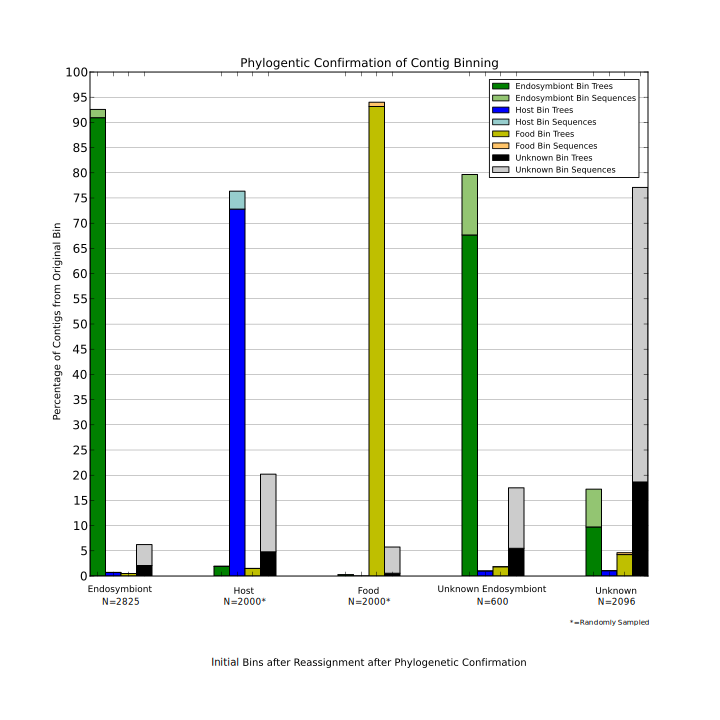
\includegraphics[width=\textwidth]{change_in_binning_after_phylogenetic_confirmation.pdf}
    \caption[Preliminary transcript binning analysis]{Preliminary analysis of change in binning after manual phylogenetic confirmation.
    	This analysis was based on an earlier iteration of the assembly and ORF calling.}
\end{figure}

\subsubsection{Phylogeny-based bin classification}
The 70,095 transdecoder called peptide sequences were then run through
the automatic phylogeny generation pipeline (``Dendrogenous'') against the 40
representative genomes described above. 
Of these, 38,193 had no BLAST hit against any genome database sequence and thus were
not used to generate phylogenies.  A further 9,335 had less than 4 hits 
and thus were not used to generate phylogenies but were taxonomically sorted based
on the BLAST hit binning criteria to give 8,574 ``host'' sequences,  258 ``endosymbiont'',
395 ``food' and 108 ``unknown''.   
An additional 9 sequences had insufficient numbers of sites 
when masking to generate a phylogeny (\(\leq30\)).  Finally, 10 phylogenies
were malformed due to a latent bug in FastTree2.  
Therefore, 22,672 phylogenies were successfully generated and named from the input sequences.
\footnote{However, in speed testing ``Dendrogenous'' did prove very efficient at rapidly generating phylogenies with its
	fully parallelised mode capable of generating 100 phylogenies randomly selected transcripts against 41 genomes in an average 2:22.50 minutes.
	The same pipeline run serially took an average of 23:41.39 minutes and the stage-wise parallel was very marginally faster at 
	an average of 21:45.02 minutes.}

The training dataset and test datasets were visualised to ensure that the training dataset 
(generated during a previous iteration of these analyses) was representative of the 
test dataset.   These plots demonstrate a possible under representation of ``Unknown'' and/or ``Food'' samples (\cref{fig:radvis_training}) but do reflect a training dataset that largely encompasses a good quantity of the same
feature space as the test dataset (\cref{fig:radvis_test}).

\begin{figure}[h!]
		\centering
		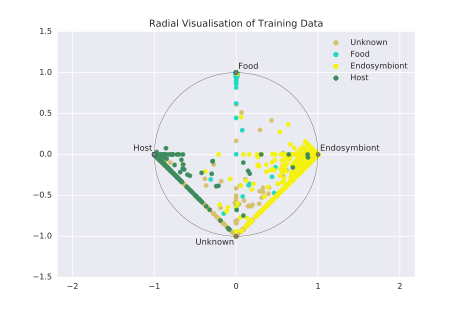
\includegraphics[width=\linewidth]{radviz_training.pdf}
        \caption[Radial visualisation of training data]{Radial Visualisation of Manually Parsed Training Data. All input features are normalised to 
			unit magnitudes.  Each point represents a single training sample (i.e. phylogeny) and its relative proximity
			to the cardinal points of the unit circle represents a the number of closely related taxa considered part of
			that ``class''.  Unknown and Food classes can be seen to be particularly problematic and poorly partitioned.
			represents the}
		\label{fig:radvis_training}
	\end{figure}

\begin{figure}[h!]
		\centering
		\includegraphics[width=\linewidth]{radviz_traing_test.pdf}
        \caption[Radial Visualisation of Test and Training Data]{Radial Visualisation of Test Data and Training Data. All input features are normalised to 
			unit magnitudes.  Each point represents a single training sample (i.e. phylogeny) and its relative proximity
			to the cardinal points of the unit circle represents a the number of closely related taxa considered part of
			that ``class''. 
			Test shows the position of all unlabelled phylogenies.  This plot shows where the training 
			data is poorly sampled - specifically phylogenies that only contain ``host'' and ``food'' taxa or
			``host'' and ``endosymbiont'' taxa.  These phylogenies may prove problematic to easily classify.}
		\label{fig:radvis_test}
\end{figure}


The large range of classification algorithms were fitted to this training dataset and
hyperparameters were efficiently optimised using random search and Bayesian optimisation on
the cross-validation folds. The average F-1 scores across classes were tallied and compared 
revealing K-Neighbours the most effective classification algorithm for this dataset (\cref{fig:f1_scores}).

\begin{figure}[h!]
	\centering
	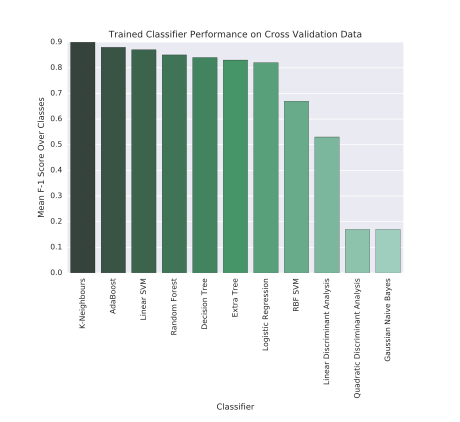
\includegraphics[width=0.8\textwidth]{sklearn_f1s.pdf}
    \caption[F1-scores of different classifiers]{Classification report must be straightforward - a report of P/R/F-Measure for each element in your test data. In Multiclass problems, it is not a good idea to read Precision/Recall and F-Measure over the whole data any imbalance would make you feel you've reached better results. That's where such reports help.}
	\label{fig:f1_scores} 
\end{figure}


As can be seen in the confusion matrix (and manual parsing of the classification reports
from each classifier (see appendix <++>)) K-neighbours (like the majority of classifiers)
poorly classified ``Unknown'' samples but largely performed well (\(0.89-0.9\) for each class
(\cref{tab:classification_report}). 

\begin{figure}[h!]
	\centering
	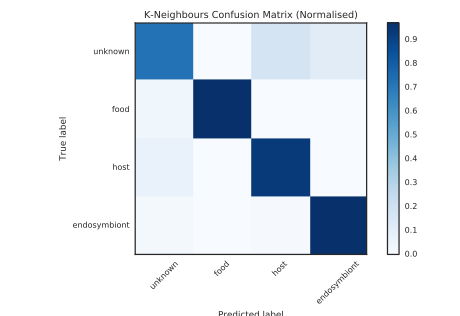
\includegraphics[width=0.8\textwidth]{kn_confusion_matrix.pdf}
    \caption[Normalised confusion matrix of transcript classification]{Normalised Confusion Matrix for K-Neighbours.  These plots highlight
		the problematic classes in the cross-validation dataset. 
		 The heatmap corresponds to the proportion of samples classified
		 with a given predicted label compared with their true labels.
		``Host'' samples are accurately classified however a small number are erroneously
		classified as ``Unknown''.  Similarly, ``Unknown'' samples are relatively poorly
		classified in general.}
	\label{fig:confusion matrices} 
\end{figure}


\begin{table}
    \centering
	\begin{tabular}{|c|c|c|c|c|}
		\hline
		\textbf{Label} & \textbf{Precision} & \textbf{Recall} & \textbf{F1-Score} & \textbf{Support} \\
		\hline
		``Unknown'' & 0.96 & 0.84 & 0.90 & 156 \\
		``Food'' & 0.98 & 0.99 & 0.99 & 426 \\
		``Host'' & 0.90 & 0.99 & 0.98 & 787 \\
		``Endosymbiont'' &  0.97 & 0.99 & 0.89 & 359 \\
		\hline
		average / total & 0.95 & 0.96 & 0.95 & 1728 \\
		\hline 
	\end{tabular}
    \caption[Classification Report for K-Neighbours]{Classification report of a trained and optimised 
	K-Neighbours Classifier using a leaf size of 30, minkowski
	distance metric and 50 neighbours.  Note the poor performance
	on ``Unknown'' samples but generally good (\(\geq90\%\)) on
	other labels. This can likely be explained by the ``miscellaneous''
nature of this label and the diverse phylogenies that comprise it. }
\label{tab:classification_report}
\end{table} 

When the trained K-Neighbours model was used to classify 
the unlabelled 22,672 phylogenies: 415 were ``endosymbiont'',
2253 ``unknown'', 19476 ``host'' and 531 ``food''. 

Therefore, of the 70,095 called ORFs in total there were:
28,050 were ``host'' derived,  
673 ``endosymbiont'',  40446 ``unknown'' and 926 ``food''.

\subsubsection{Performance relative to TAXAssign}

TAXAssign performed relative poorly at taxonomic classification/binning
of transcripts.  Of 70,605 CDS sequences only
2,043 (\(2.893\%\)) were assigned a phylum level taxonomic identity (\cref{tab:taxassign}).

Of these top level assignments:
\begin{table}
    \centering
	\begin{tabular}{| c | c | c |}
\hline
\textbf{Class} & \textbf{Phylum} & \textbf{Sequences Assigned} \\
\hline
``Host'' & Intramacronucleata & 97 \\
``Endosymbiont'' & Streptophyta & 101 \\
				 & Chlorophyta & 58 \\
				 & Cyanobacteria & 1 \\
``Food'' & Proteobacteria & 1270 \\
	& Firmicutes & 80 \\
	& Actinobacteria & 35 \\
	& Bacteriodetes/Chlorobi & 29\\
``Unknown'' & Chordata & 365 \\

& Chlorovirus & 94 \\ 
			& Arthropoda & 7 \\
			\hline 
	\end{tabular}
    \caption[TAXAssign Taxonomic Assignments]{Phylum level TAXAssign assignments for (\(2,043/70,605\)) CDS called from the Bridger 31-mer assembly.
            Only \(2.893\%\) were assigned using this method relative to  \(39.72\%\) for 
        the phylogenetic supervised learning (Dendrogenous-Arboretum) method.  Therefore, this demonstrates the
        the how well this method works relative to conventional binning approaches like TAXAssign.}
	\label{tab:taxassign}
\end{table}

This can be contrasted with the 29649/70605 or \(41.99\%\) classified 
using the phylogeny and supervised classification system..

\section{Discussion}

\subsection{Library screening is a key stage in sc-RNAseq}

Despite evidence and hope that nanoscale methods can greatly reduce levels of contamination \citep{Blainey2011}, 
the taxonomic profiling conducted here
indicates a high level of bacterial (and viral) contamination in the scRNA-Seq.  
Therefore, much as library contamination is one of the key issues with single cell genomics \citep{Blainey2013,Lusk2014}, it is also highly
important in SCT.  This is in concordance with the findings of \citep{Kolisko2014}, 
in which enigmatic, bacterial contamination was a problem in single cell eukaryotic
transcriptomes.   

Single cell methods are particularly prone to contamination issues
from reagents, laboratory environment and enigmatic nucleic acids within the biological samples themselves.
This is due to the low-input concentration and high amplification necessary in these approaches \citep{Blainey2013} 
leading to enrichment of non-target sequences, especially bacterial contaminants present around or within the
\textit{P. bursaria} host.  
It is critical to identify and discard highly contaminated libraries in \textit{de novo} assemblies as contaminant
reads severely complicate the assembly graph thus increasing the computational difficulty and reducing the accuracy
of the de-Bruijn graph path resolution.  This was highlighted by observations in the preliminary 
stages of this project that the inclusion of certain (SCT) libraries would increase
assembly run-time and lead to the generation of fragmented transcripts relative to assemblies without those
libraries.  

Taxonomic profiling also reveals other features of the dataset that wouldn't necessarily be
obvious otherwise.  For instance, our profiles revealed systematically low 
low levels of Viridiplantae related reads across both bulk and sc-RNAseq libraries and in both lit and dark conditions.  
Despite care being taken to ensure thorough lysis of the chitinous \textit{Micractinium} cells during 
RNA extraction and a ratio of \(\sim 300:1\) endosymbiont to host cell ratio this may be related to lytic inefficiencies \citep{Korfhage2015} or potentially
just relatively fewer endosymbiont transcriptomic activity relative to host and associated bacteria species.
Finally, it is possible that due to the endosymbiont being largely provisioned by the host it may be relatively
transcriptionally inactive and thus relatively fewer transcripts can be recovered. 



Intriguingly, taxonomic profiling of the bulk libraries showed a very low percentage of reads 
mapping to any sequence in the nr protein database.  This was significantly lower than the
sc-RNAseq libraries.  While this finding is concerning it is likely to be an artefact of the older 
sequencing platform the bulk data was generated on.
These paired reads were sequenced via the GAII and were half the length of the HiSeq2500 reads used for 
the SCTs.  Shorter reads and a relatively higher
technical error rate on this platform may have played a role in this marked decline in recognisable reads. 
Despite this the relative proportion of bacterial reads to eukaryote reads among the 
recognisable reads is much lower for bulk libraries than SCT.  This does however suggest, that
read length is highly important to accurate contamination screening/taxonomic profiling.

Taxonomic profiling of reads/libraries proved surprisingly robust to trimming.  The profiles
generated in ``DueyDrop'' were largely identical regardless of whether the input library 
had been trimmed or not (even at high stringency thresholds).  This indicates that
screening can occur before the computationally expensive trimming process without loss
of accuracy.   
While the results presented here demonstrate that the profile
generated from a relatively small random subsample of a library is largely consistent 
with that of the profile generated from the library as a whole.
 
``DueyDrop'' could potentially be improved in such a way that an entire library can be screened quickly instead of just subsamples.
Briefly, this would involve quantifying exact K-mer matches between library reads and a pre-generated database of known taxa
using efficient probabilistic hashing data structures such as a bloom filter, or more likely count-min sketch and an efficient
k-mer counting library such as Jellyfish \citep{Marcais2011}.  This would have a major speed advantage compared to the BLASTX-based method of ``DueyDrop''
and would thus allow entire libraries to be checked in reasonable time.  A similar approach to this has been implemented as a service
by \url{https://www.onecodex.com/}, although this focuses specifically on screening for medically relevant taxa. 
However, it would require laborious workarounds to handle
K-mers shared between multiple taxa in the database, translation of reads and/or database sequences into a matching sense and form (e.g. protein),
and use of a locality-sensitive hash function to handle scenarios where there is no exact k-mer match. This latter issue is particularly
problematic for libraries consisting of transcripts from poorly sampled sections of the tree of life where exact matches would become
commensurately rarer as sampling sparsity increases.  
While still affected by this problem, the BLASTX/Diamond approach implemented in the ``DueyDrop'' scripts are relatively more robust to these
problems due the explicit probabilistic modelling of sequence divergence built into the BLAST alignment algorithm (e.g. E-values).
Other potential improvements to ``DueyDrop'' would be to incorporate some degree of 
automatic clustering of phylogenetic profiles using unsupervised learning and possibly manifold embedding, potentially
including a form of anomaly detection to discover contaminated libraries.  
Robustness of taxonomic inference for each profile can also be improved by taking all hits instead of just the top one
and resolving conflicting phylogenetic signal using a lowest common ancestor algorithm over all the hits.

\subsection{Combining single cell and bulk transcriptome data creates new challenges}

Contrary to previous studies in optimising conventional RNA-seq assemblies where:
permissive trims \citep{Macmanes2014}, error correction \citep{Macmanes2013,Macmanes2015} and the combination of multiple assemblies
\citep{Nakasugi2014} have been demonstrated as effective tactics in recapitulating a comprehensive
set of transcripts \textit{de novo}, MDA-based SCT and bulk datasets such as the one investigated
above exhibit different properties.  
It is important to pick a trimming threshold which minimises sequence error (mostly substitutions \citep{Yang2013}) as these
result in assembly of spurious sequences but doesn't discard reads necessary to complete transcripts \citep{Macmanes2013,Macmanes2014}. 
For the \textit{P. bursaria} - \textit{M. reisseri} bulk and SCT dataset the optimal trimming threshold - based on both
mapping statistics to preliminary assemblies and final assembly likelihoods proved to be a harsh threshold of Q30. 

Following a similar theme, despite numerous indications that error correction is important for improving the accuracy
of genomic and transcriptomic assemblies using Illumina reads (e.g. \citep{Molnar2014,Macmanes2015}) 
in the case of this dataset error correction appeared to be have a minimal effect with few
reads being corrected and downstream assemblies being largely equivalent to those
without error correction.  In fact, permissively trimmed (Q5), error corrected assemblies 
were shown to have lower likelihoods and smaller assembly sizes
than more conservatively trimmed assemblies (Q30).
It should be noted that SEECER, while an RNAseq specific error correction tool is not
optimised for single cell MDA-based datasets, and Bayeshammer is not optimised
for transcriptomic data.  Therefore, the poor performance of error correction
in this dataset might be a consequence of the lack of error correction tools
designed for MDA-based sc-RNAseq datasets. It will likely prove beneficial, as 
datasets of this type become more prevalent, to develop tools for this specific
use case combining the most effective features of the MDA aware BayesHammer 
and the RNA-seq optimised SEECER.  This said, there are several other available 
Illumina RNA-Seq error correction tools 
which were not trialled, ``SEECER'' was chosen in accordance to the recommendations based on dataset and hardware
heuristics (\(>50M\) reads and the availability of a high memory system) \citep{Macmanes2015} but
as we've demonstrated the limitations of such heuristics on new types of data it might 
be worth investigating these alternative tools further.

Finally, merging multiple assemblies proved a sub-optimal strategy with all
merged assemblies generating lower likelihood assemblies than the
best individual assembly.  While not merging assemblies might mean specific
transcripts might not have been recovered, especially assemblies at a range
of K-mer sizes (short K-mers generally recover lower expression transcripts
and vice versa for long K-mers), the much higher likelihoods meant the
best performing individual assembly (Bridger using 31-mers, Q30 trimmed
taxonomically selected SCT and bulk libraries) was preferred.

These results suggest that MDA-based single cell transcriptomic datasets
do not behave in a qualitatively similar way to bulk RNA-seq in terms of
pre-processing and assembly parameters.  
This means care must be taken incorporating advice and heuristics
derived from studies based on analysis bulk RNA-seq datasets (e.g. \citep{Macmanes2013,Macmanes2014,Macmanes2015,Nakasugi2014}).
As further studies using MDA SCTs are completed (e.g. \citep{Kolisko2014}) 
a greater understanding of the optimal analysis of this type of 
dataset will emerge.

\subsection{Pre-assembly read partitioning is non-trivial}

As we expect the PbMr metatranscriptome to contain predominantly a highly AT-rich organism, \textit{Paramecium},
(ranging from 24.1 to 28.2\%GC in \textit{P. aurelia} species complex and \textit{P. caudatum} \citep{Aury2006,McGrath2014})
and a very GC-rich organism, \textit{Micractinium}, (\textit{Chlorella variabilis} NC64A genome is approximately 67.1\%GC, the highest
found in a sequenced eukaryote genome (in 2010) \citep{Blanc2010}), the utility of pre-assembly read partitioning was assessed.
This GC pattern was supported by the clear bimodal GC distribution that can be observed in \cref{fig:gc_prop_raw}.
However, under careful observation it was apparent that the bimodal GC distribution was more attributable to 
the presence of a GC-rich contaminant such as Rhizobiales \citep{Peralta2011}.  Therefore, in practice pre-read partitioning was mainly attempted to 
try to remove these contaminant reads from screened libraries.
Theoretically, accurate pre-assembly read partitioning could transform a complex assembly graph into two relatively simpler
assembly tasks.  As well as simplifying path resolution accuracy, if this method could
 speed up assembly considerably and thus allow more iterations to optimise other
assembly parameters.

This pre-assembly partitioning has been tried with mixed success in other meta-omic analyses (e.g. \citep{Droge2012}).
However, a lack of fast efficient tools to accomplish this led to the creation of ``parKour''.
The developed GC partitioning package proved very effective at rapidly and relatively computationally 
efficient clustering of PE RNAseq data. ParKour generated clusters with centroids
reasonably where they may be expected from inspection of per read GC probability densities (see \cref{fig:gc_prop_q30})
i.e. partitioning out the GC rich potentially contaminant reads likely from \textit{Rhizobia}
bacterial species.  Unfortunately, in the case of this dataset clustering proved ineffective
at improving assembly accuracy and fully removing groups of contaminant reads with large GC skews. 
The likely explanation for this is that even 150bp paired end reads are too short to consistently
statistically demonstrate the GC-AT bias of the originating organism. This means any partitioning
is likely to remove a significant number of reads necessary to complete transcripts due to local
variation in AT bias.  The high number of shorter contigs is indicative of the kind of assembly
fragmentation that would be expected in this situation.

However, the relative efficiency and theoretical benefits of this type of clustering indicates there may be
some potential to utilising a similar but less naive approach in future work.
It may be possible to combine ``DueyDrop'' and ``ParKour'' to all
read-level screening and partitioning of reads on the basis of taxonomic profile
and compositional characteristics such as GC\% and tetramer frequencies.
This could improve resolution of clusters and decrease the observed contig fragmentation
effect while performing accurate taxonomic screening. 

Other improvements could include the consideration of alternative clustering algorithms 
such as k-medoids \citep{Kaufman1987} with more robust outlier stability or large scale
database clustering algorithms such as DBSCAN \citep{Ester1996} or BIRCH \citep{Zhang1996} (allowing non-convex
clusters). Silhouette coefficients and analysis\footnote{
	\(s = \frac{b -a}{max(a,b}\) where \(s\) is Silhouette coefficient, \(a\) is the mean distance
	between a sample and all other points in the same class and \(b\) is the mean distance
	between a sample and all other points in the next nearest cluster \citep{scikit-learn}.  Therefore,
	\(s\) is a measure of cluster definition.}
\citep{Rousseeuw1987} can be incorporated to aid determination of the expected number of clusters when it cannot be determined
\textit{a priori} from inspecting the data as well as validation of generated clusters.  
Unfortunately, other validation and analysis systems are somewhat limited due to the lack of ground truth labelling 
available.  
Alternatively,
a variational Bayes approach could be implemented to determine the optimal number of clusters (e.g. CONCOCT \citep{Alneberg2014}).
Finally, memory efficiency can be improved by use of streaming clustering algorithms (e.g. those discussed in
\citep{OCallaghan2002})
in which all data does not require to be loaded into a matrix at a given time and be clustered
as they are parsed.  

\subsection{Digital normalisation greatly improves assemblies}

Digital normalisation, a method to remove redundant read data from libraries and thus
reduce the computational burden of assembly \citep{Brown2012}, was also investigated for this dataset
and found to be a highly effective strategy in improving assemblies of mixed bulk and MDA SCT data.

Interestingly, some have argued that error correction is special case of general digital normalisation
\citep{Krasileva2013}.  This is supported by the fact that many error correction
algorithms operate on similar principal of attempting to remove low abundance K-mers
from input datasets. K-mers with a low abundance
are more likely to be due to sequencing errors than representing novel biological
diversity.   
This said digital normalisation has the potential to
spuriously discard true variation that is merely undersampled in our libraries
due to the high level of contamination.  

This hypothesis is somewhat supported by the disproportionate 
retention of bulk reads relative to noisy single cell reads.  However,
within the context of the single cell reads the more highly
contaminated Dark reads were retained in roughly equal proportion to the light reads.
Suggesting, MDA derived data may also just display a greater quantity of 
low-level sequencing error.  

It should be noted that the digitally normalised and K-mer abundance filtered assemblies also
incorporated more bases overall than the equivalent assembly using the full
libraries therefore resultant assemblies were just high confidence (and likelihood)
subsets of the initial input data.

One factor that has not been adequately analysed in the context of this work
is that of sequencing depth.  Future studies will need to carefully consider
sufficient sequencing depth given the noise and prevalence of contamination
in MDA based data.


\subsection{Assembly and assembly assessment}

While we have demonstrated that some progress can be made 
identifying optimal pre-processing parameters using measures such as mapping metrics 
it is very difficult to identify the parameters (preprocessing or otherwise) which will leads to the ``best'' 
\textit{de novo} assembly without actually generating the assembly.
  Assembly can be considered an example of Wolpert and Macready's ``No Free Lunch Theorems'' \citep{Wolpert1995,Wolpert1997} 
  as (in the case of \textit{de novo} assembly) it is fundamentally a hamiltonian/eulerian cycle search problem (equivalent
    in the de-Bruijn formulation) and therefore any two assembly implementations (in different assemblers and/or
    with different parameters) should ultimately be equivalent across all possible input datasets.\footnote{
    This should be taken with a pinch of salt, a proof of this theorem applied to the case of assembly is beyond
both the scope of this thesis and my abilities}.  For this reason, it is necessary to try
assembly using a random of assembly parameters and indeed a range of both \textit{de novo} and referenced assemblers. 

Unfortunately, the task of identifying the ``best'' \textit{de novo} transcriptome assembly is also a non-trivial 
task \citep{Neil2013c}.  Many widely used assembly assessment metrics have been shown to be
inconsistent measures in simulated sequencing data, especially those metrics related to individual
contigs (theoretically different transcript splices).  Metrics such as average length and N50
prove consistent across both simulated sequencing depth and read lengths i.e. they improve 
towards \citep{Neil2013c}.  Furthermore, the number of possible metrics is greatly reduced
if assessment is mainly conducted in a reference-free manner \citep{Li2014}.  As the majority of
assemblies were \textit{de novo} and the suitability of the related but divergent genomes
proved lacking it was necessary to restrict to reference-free assembly assessments.  
Therefore, a model-based reference-free assembly scoring algorithm (RSEM-EVAL \citep{Li2014} was,
 along with standard (if imperfect) metrics, used to evaluate different assemblies in this study.
 The assumption of the accuracy of the RSEM-EVAL likelihood is a strong one, and deserves careful re-consideration
 in further work.

In terms of referenced assembly using divergent relatives, 
it is safe to conclude that despite other findings that even divergent 
(up to 15\%) genomes can generate transcriptomes of higher-quality
than \textit{de novo} \citep{Vijay2013}, the potential references
are too divergent in the case of the PbMr to be of any utility.
    
Overall, a comparison of \textit{de novo} assemblies
using a range of assemblers and parameters on ``optimally'' pre-processed
read data demonstrated the clear superiority of both ``Bridger'' and ``Trininty''
Trinity comes with the advantages of being a generally better developed tool that interlocks effectively via several plugins and utility
scripts with other tools and analysis pipelines.  

However, despite being relatively newer and consisting of
a less mature and tested codebase, Bridger proved to be
a slightly more effective assembly tool overall. Unfortunately,
coding problems and a lack of public active development means 
it is non-trivial to successful use this tool.  In the process of 
implementing the above analyses it was necessary to fix several
bugs present in the assembler. These upgrades were merged into
the code and are available on GitHub \url{https://github.com/fmaguire/Bridger_Assembler}.
Hopefully, by rehosting this code on a public development and collaboration
platform (as well as adding continuous integration) will 
spur further development of this promising tool.


Interestingly, despite strong evidence supporting the need to combine assemblies due to the 
size of the disjoint sets of transcripts recoverable from different algorithms and parameter
choices \citep{Lowe2014} assembly merging systematically led to worse overall assemblies
with this dataset (as assessed by RSEM-EVAL likelihood scores).  The likelihood of the merged
assemblies were worse than the best individual constituent assemblies.


\subsection{Binning}

However, even once a good assembly has been generated it is still necessary to identify the likely
originating species of a given transcript i.e. host, endosymbiont, food bacterial contaminant or other
contaminant.  While a successful partitioned pre-assembly strategy may simplify this process it would still
be sensible to confirm bins using downstream analyses that use full length assembled transcripts and thus
more potential data than are present in shorter individual PE reads.  Rough, approximate bins were
generated using a simple "top BLAST hit" approach following ORF calling (using Tetrahymena and Universal
encodings) against a set of representative predicted proteomes.  In order to assess how accurate these
bins were likely to be, 10,000 were randomly selected and rapid maximum-likelihood phylogenies were
generated using the transcript sequence as a seed to sample the entire RefSeq protein nr database.
This was accomplished using ``Dendrogenous'', a rewritten and modified version of a pipeline originally known 
as ``Darren's Orchard'' which first appeared in \citep{Richards2009g}.  Phylogenies were manually assessed to check
whether the resultant topology was congruent with the BLAST based binning i.e. are supposedly ``endosymbiont''
transcripts branching principally with archaeplastida taxa.  
However, due to the slow largely manual nature of this phylogeny assessment process it would be infeasible
to repeat this for all transcripts generated from a single assembly, let alone investigating several. 

Therefore, this became a fundamental classification problem with the 10,000 manually verified phylogenies
forming a handy training dataset for supervised learning.   To determine the best performing
classification algorithm and hyperparameters for this dataset an automated search was conducted 
using bayesian optimisation.  This was then converted to a binning script named ``Arboretum''.
High throughput phylogeny generation, parsing and supervised classification is 
a more sensitive and powerful way in which to bin transcripts into their likely originating
organisms provided a reasonable level of \textit{a priori} knowledge of the system at hand.
This demonstrably operates better than established although simpler approaches such as
TAXAssign or top BLAST hit.  While, classification accuracy (and F-1) is sub-optimal 
for ``Food'' and ``Unknown'' bins it (\cref{tab:classification_report}) a decent level of 
precision and recall for the target bins of ``Host'' and ``Endosymbiont''.

However, this classification
is still a work in progress and could potentially be improved by the 
addition of anomaly detection in place of the catch-all (and subsequently poorly classified)
``Unknown'' classes.  Furthermore, there are several potential possible improvements
in the classification itself that could be made.
Specifically, unsupervised clustering pre-training could potentially
forgo the need for laborious manual generation of the training dataset and minimise 
the difficulties in handling these aberrant phylogenies.
An AutoML bagging estimator such as one of those implemented in the AutoML project \citep{Eggensperger2013}, 
a variational autoencoder pre-processing following by a 
deep neural network classifier or using a phylogeny specific kernel 
function \citep{Vert2002} in a Gaussian process or
SVM system all offer potential algorithmic improvements.
Finally, incorporation of additional sequence related features such as
K-mer coverage and composition into each samples may help greatly improve
the fidelity of classification.

\section{Conclusion}
In conclusion, for this dataset the optimal pre-processing
was determined to be careful taxonomic screening of input libraries,
followed by trimming at a high (Q30) threshold and subsequent
digital normalisation and low-abundance K-mer filtering. 
The optimal assemblies were generated using larger (25-31 K-mer)
sizes and utilised the Bridger (and to lesser extent Trinity)
assembly algorithms.  While pre-assembly read partitioning proved 
ineffective in this implementation, in future a less naive
method that incorporated both read-level taxonomic data and
compositional information could potentially improve assemblies of 
complex eukaryotic metatranscriptomes, especially those that
combined bulk and single cell RNAseq data.  Generally,
MDA-based single cell datasets are noisy and difficult to work with.
Potentially, they require the existence of robust references to aid
assembly or a much greater depth of sequencing.

Finally, I have demonstrated that BLAST based transcript binning alone is
ineffective at accurately binning transcripts. Fast, automated phylogeny generation
and the subsequent use of supervised learning (particularly
large ensemble models such as Random Forests and those AutoML algorithms)
can potentially improve the quality of such binning.  Further work 
in the implementation of unsupervised clustering of generated phylogenies
could conceivably forgo the laborious process of manually generating
a training dataset.

\begin{table}
\centering
\begin{tabular}{|c|c|c|}
        \hline
        \textbf{Transcript Bin} & \textbf{Number of Transcripts} & \textbf{Called ORFs} \\
        \hline
        Endosymbiont  & 8,975 & 4,275 \\
        Host & 18,793 & 17,920 \\
        Food & 18,516 &  - \\
        Unknown & 66,107 & - \\
        \hline
\end{tabular}
    \caption[Summary of Transcriptome Bins]{Summary of transcriptome assembly and binned sequences}
    \label{tab:bin_assem_summary}
\end{table}

Points arising in this analysis:
\begin{itemize}
    \item It is possible to generate a functional working transcriptome combining bulk and MDA based RNAseq (see \cref{tab:bin_assem_summary})
    \item sc-RNAseq libraries generated from dark samples are problematic.
    \item Binning methodologies may prevent easy finding of novel genes due to a lack of homology. 
\end{itemize}


